%!TEX root = ../Thesis.tex

\chapter{Experimental work}\label{chp: Experimental results}
% Qoute ...
\chapterquote{It is shown that many particular choices among possible neurophysiological assumptions are equivalent, in the sense that for every net behaving under one assumption, there exists another net which behaves under the other and gives the same results, although perhaps not in the same time.}{McCulloch, W.S. and Pitts, W. H. (1943) \cite{McCulloch1943}}

%!TEX root = ../Thesis.tex

\section{Introduction}
In addition to the theoretical work presented in the preceding chapters, this thesis has spent some effort on implementing and experimenting with the different methods, algorithms and augmentations. The algorithms have been implemented in Python using parts of the PyTorch deep learning library.
Brief explanations and references to full code repositories are given in \autoref{app: implementations of algorithms}. The experiments were run on the \gls{HPC} cluster at DTU. This section presents the results of the experimental work. 

\autoref{sec: Experimental work: Benchmarking} presents the problems used for the benchmarking and while the different \gls{NN} architectures used are described in \autoref{sec: Experimental work: Neural network architectures}. 
The general computational complexity and scaling properties of the \gls{VO} algorithm are examined for both a supervised problem and a reinforcement learning problem in \autoref{sec: Experimental work: Computational scaling}.
\autoref{sec: Experimental work: Effects of common model and algorithm augmentations} examines the influence of the model augmentations of batch normalization and dropout along with safe mutation.
In \autoref{sec: Theory: Methods for variance reduction}, the different methods for reducing the variance of the gradient are examined- This includes gradient momentum in \ref{sec: Experimental work: Effect of momentum} and antithetic sampling in \ref{sec: Experimental work: Antithetic sampling}.
Finally, the effect of adapting the variance using different Gaussian search distributions is evaluated in \autoref{sec: Experimental work: Effect of adapting the variance}.

It should be noted that the number of hyperparameters combined with variations on the \gls{VO} algorithm gives a large number of potential experiments to conduct. This thesis has only performed a small subset of all the possible experiments. The chosen experiments were selected based on what had the highest potential to show improvement to the algorithm.

%!TEX root = ../Thesis.tex

\section{Benchmark problems}\label{sec: Experimental work: Benchmarking}
\subsection{Supervised learning benchmark}
Within the supervised learning setting, the classical problem of handwritten digit recognition based on the \gls{MNIST} dataset \cite{LeCun1998} was chosen. This is a small and relatively simple data set that has allowed for rapid prototyping and aided in algorithm development, historically and in this thesis. Even though it has recently received criticism for being too simple, it remains one of the most widely used benchmarks within deep learning \cite{Xiao2017}. The training data consists of 60.000 greyscale images of handwritten digits between 0 and 9 and the associated label. Each image has $28\times28$ pixels and represents a single digit. The test data consists of 10.000 images and associated labels.
In this thesis, no data augmentation has been applied to the data set. Examples from the \gls{MNIST} dataset can be seen in \autoref{fig: mnist-examples/MNIST-10x10-sorted.pdf}.
\begin{figure}[tbp!]
    \centering
    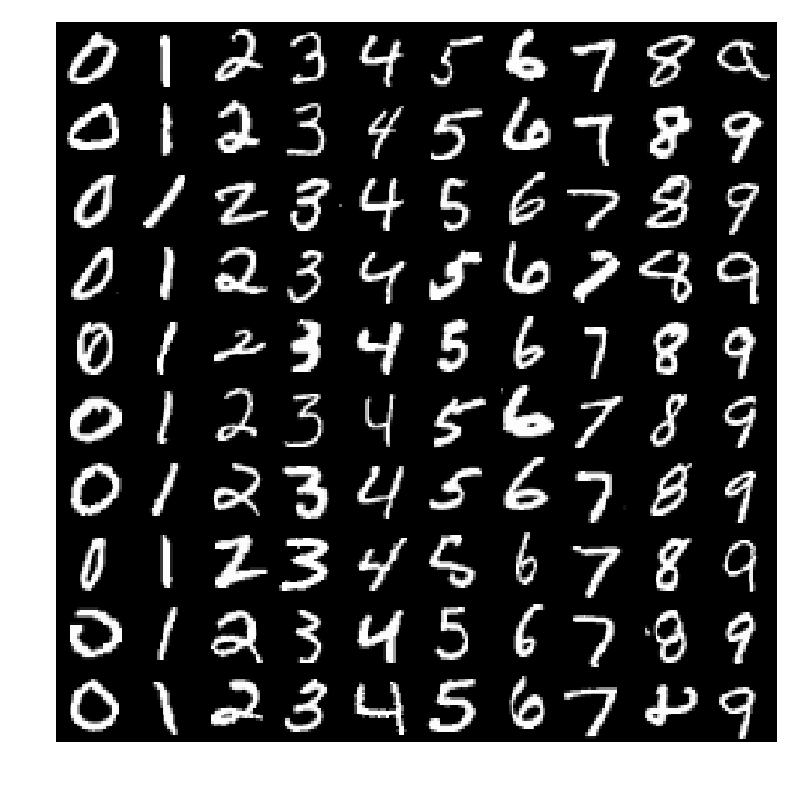
\includegraphics[width=0.60\textwidth]{graphics/mnist-examples/MNIST-10x10-sorted.pdf}
    \caption{
        Examples from the \gls{MNIST} dataset sorted by target values from 0 on the left and 9 on the right. As is well-known, a few examples from the dataset are very hard to correctly classify, note for example the bottom most 8 and the top most 9.
    }
    \label{fig: mnist-examples/MNIST-10x10-sorted.pdf}
\end{figure}

To the author's best knowledge, the currently best performing non-ensemble \gls{NN} model on \gls{MNIST} is the deep \gls{FNN} using DropConnect \cite{Wan2013, Hasanpour2016} which achieved $99.79\%$ classification accuracy also exploiting extreme data augmentation. An accuracy of $99.76\%$ was achieved in \cite{Chang2015} which uses a max-out network in network \cite{Lin2013} model with no data augmentation. Using backpropagation and the network to be used for \gls{MNIST} in this thesis (introduced in \autoref{sec: Experimental work: Neural network architectures (MNIST)} and shown in \autoref{lst: Network models: MNIST with batch normalization}) the best achievable accuracy is about $99.1\%$ using \gls{SGD} with momentum training for 20 epochs. With the Adam algorithm, accuracy can reach $99.2\%$ for 20 epochs.


\subsection{Reinforcement learning benchmarks}
Within the reinforcement learning setting, focus has been primarily on two environments from the OpenAI Gym toolkit \cite{Brockman2016}. The first environment is the Atari-2600 game of Freeway\footnote{\url{http://en.wikipedia.org/wiki/Freeway_(video_game)}, \url{http://gym.openai.com/envs/Freeway-v0/}} in which the agent controls a chicken that must be brought to pass a busy ten lane highway by moving either up or down. If hit by a car, the chicken is pushed either slightly back or moved to the starting position. A reward of $1$ is given for each successful passage and the total score is the number of passages within a time slot of $2$ minutes and $16$ seconds. In \cite{Salimans2017}, using a the fixed variance \gls{ES} similar to \gls{VO}, a score of $31$ was achieved when averaged over 10 re-runs with the DQN network of \cite{Mnih2016} encoding a deterministic policy. This network is also used for \gls{RL} in this thesis

The second \gls{RL} environment is the Atari game of Seaquest\footnote{\url{http://en.wikipedia.org/wiki/Seaquest_(video_game)}, \url{http://gym.openai.com/envs/Seaquest-v0/}}. Here, the agent controls a submarine which must fend off enemies using torpedoes while rescuing divers by moving to their location. The submarine's oxygen supply is limited and the agent must occasionally bring it to the surface to refill and to receive points from rescued divers. The submarine can move in four directions and fire torpedoes. Seaquest is considered harder than Freeway due to the larger action space and more complicated objective. In \cite{Salimans2017}, a score of $1390.0$ was achieved in the same way as for Freeway.

In this thesis, \gls{VO} is used to optimize a policy which maps from the environment's observation space to its action space. The policy is parameterized by a \gls{NN} model, in this case also called a policy network \cite{Silver2014}. The policy is deterministic in that the most probable action, as computed by the policy network, is always taken. Due to computational limitations, the number of experiments made in the reinforcement setting is fewer than in the supervised setting.

In general, hyperparameter optimization has been performed manually and heuristically. Ideally, random hyperparameter search \cite{Bergstra2012a} would have been employed to find optimal hyperparameters but was not due to limited computational resources.


\subsection{Preprocessing of MNIST}
Although no data augmentation is applied to the \gls{MNIST} dataset, the data is normalized before being input to the \gls{NN}. That is, for each digit image, the average pixel value is computed along with the variance and these are aggregated to a mean and variance for the full dataset. For \gls{MNIST}, this could be done in a single computation since the entire data set fits in memory. However, since larger datasets were also tried out, the computation was implemented in an online manner according to the algorithm proposed by \cite{Welford1962}. 

The algorithm consists of updating the mean as usual and the variance through online updates to the squared sample distance from the mean. For the mean
\begin{equation}
    \bar{x}_n = \bar{x}_{n-1} + \frac{x_n-\bar{x}_{n-1}}{n} \ .
\end{equation}
% \begin{align*}
%     \bar{x}_n
%     &= \frac{1}{n}\sum_{i=1}^n x_i\\
%     %&= \frac{1}{n}\pa{\sum_{i=1}^{n-1} x_i + x_n}\\
%     &= \frac{n-1}{n}\frac{1}{n-1}\sum_{i=1}^{n-1} x_i + \frac{1}{n}x_n\\
%     &= \frac{n-1}{n}\bar{x}_{n-1} + \frac{1}{n}x_n\\
%     &= \bar{x}_{n-1} + \frac{x_n-\bar{x}_{n-1}}{n} \ .
% \end{align*}
%which can be written as
%\begin{equation}
%    \bar{x}_n = \bar{x}_{n-1} + \frac{x_n-\bar{x}_{n-1}}{n} \ .
%\end{equation}
Likewise, the update for the variance is
\begin{align*}
    s^2_n
    &= \frac{(n-2)}{(n-1)} s^2_{n-1} + \frac{(x_n - \bar{x}_{n-1})^2}{n} \ , \quad n>1 \ .
\end{align*}
This online update of the variance is prone to numerical instability which is avoided by updating the squared sample distance from the mean
\begin{equation*}
    M_{2,n} = M_{2,n-1} + (x_n - \bar{x}_{n})^2 %(x_n - \bar{x}_{n-1})(x_n - \bar{x}_{n})
\end{equation*}
and then computing 
\begin{equation*}
    s_n^2 = \frac{M_{2,n}}{n-1} \ .
\end{equation*}
These formulas have been generalized to the case of multiple examples being added at each online update \cite{Chan1979}. Here, this is needed to avoid looping over the $28\times28=784$ pixels of each image. Let $A$ and $B$ denote two samples with $n_A$ and $n_B$ examples respectively and a mean, variance and squared sample distance from the mean denoted by $\bar{x}_A$, $\bar{x}_B$, $s^2_A$, $s^2_B$, $M_{2,A}$, $M_{2,B}$, respectively. The update formulas for the aggregated sample $X$ are then
\begin{align*}
    \delta &= \bar{x}_B - \bar{x}_A\\
    \bar{x}_X &= \frac{n_A}{n_X}\bar{x}_A + \frac{n_B}{n_X}\bar{x}_B\\
    M_{2,X} &= M_{2,A} + M_{2,B} + \delta^2\frac{n_A n_B}{n_X}\\
    s_X^2 &= \frac{M_{2,X}}{n_X-1}
\end{align*}
where $n_X = n_A + n_B$.

The computed mean and standard deviation for the \gls{MNIST} dataset were then used to normalize each input pixel $x_i$ as
\begin{equation*}
    \hat{x}_i = \frac{x_i-\bar{x}}{s} \ .
\end{equation*}


\subsection{Preprocessing of Atari environments} \label{sec: Experimental section: Preprocessing of Atari environments}
Atari environments are preprocessed in the same way as in \cite{Mnih2015}. A frame from an Atari game is a $210\times160\times3$ pixels RGB image. Due to the limited number of sprites an Atari 2600 was able to display at once, some objects in games occur only in even frames while others occur only in odd frames \cite{Mnih2015}. To remove this flickering, a single frame is encoded as the maximum value of each pixel of the most recent frame and the previous frame. The frame is then converted to greyscale and resized to $84\times84$ using a pixel area relation which gives moiré-free results, is fast and yields good results for image downsampling \cite{OpenCVDevelopmentTeam2014}. This reduces the dimensionality of the frame by more than a factor of ten from $210\times160\times3=100800$ pixels to $84\times84=7056$ pixels. The input given to the \gls{NN} model is the four most recent frames seen such that the input dimension is $4\times84\times84$. This gives the model directional information about movement in the images without the use of recurrent units.

\begin{figure}[tbp!]
    \begin{subfigure}[b]{0.32\textwidth}
        \centering
        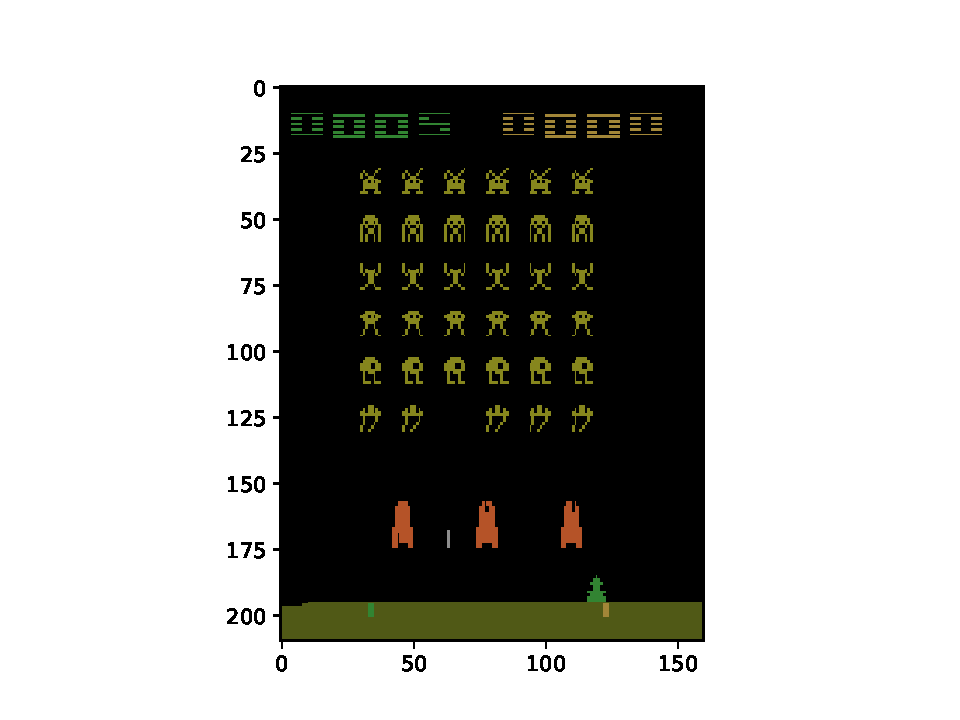
\includegraphics[height=5.8cm]{graphics/atari-pre-processing/1-spaceinvaders-original-cropped.pdf}
        \caption{}
        \label{fig: Experimental work: atari-pre-processing-1-spaceinvaders-original}
    \end{subfigure}
    \hfill
    \begin{subfigure}[b]{0.32\textwidth}
        \centering
        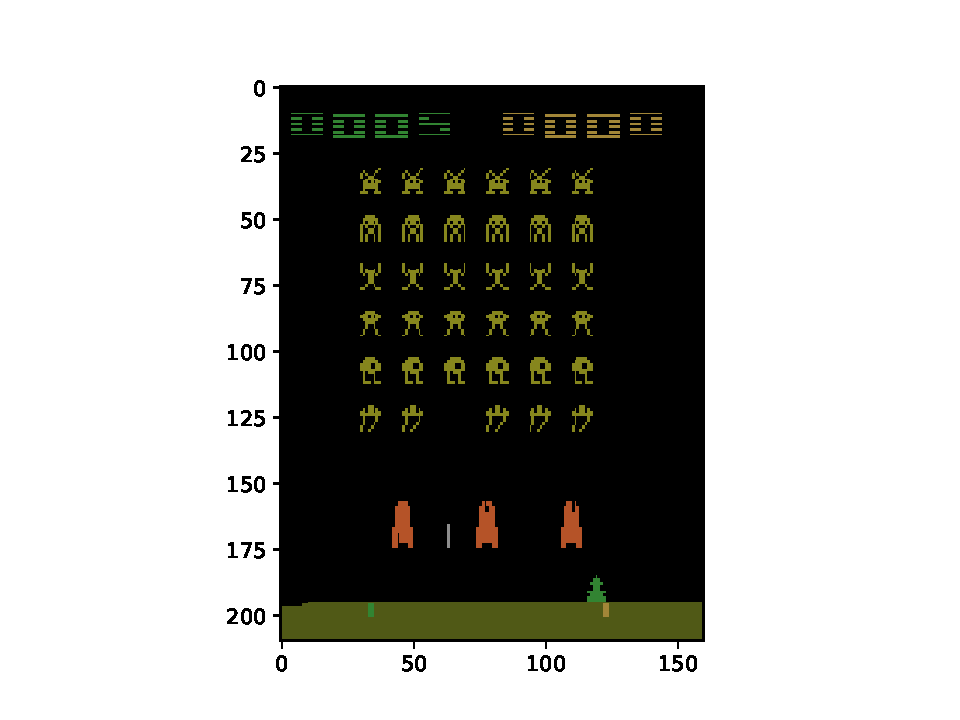
\includegraphics[height=5.8cm]{graphics/atari-pre-processing/2-spaceinvaders-flicker-cropped.pdf}
        \caption{}
    \label{fig: Experimental work: atari-pre-processing-2-spaceinvaders-flicker}
    \end{subfigure}
    \hfill
    \begin{subfigure}[b]{0.32\textwidth}
        \centering
        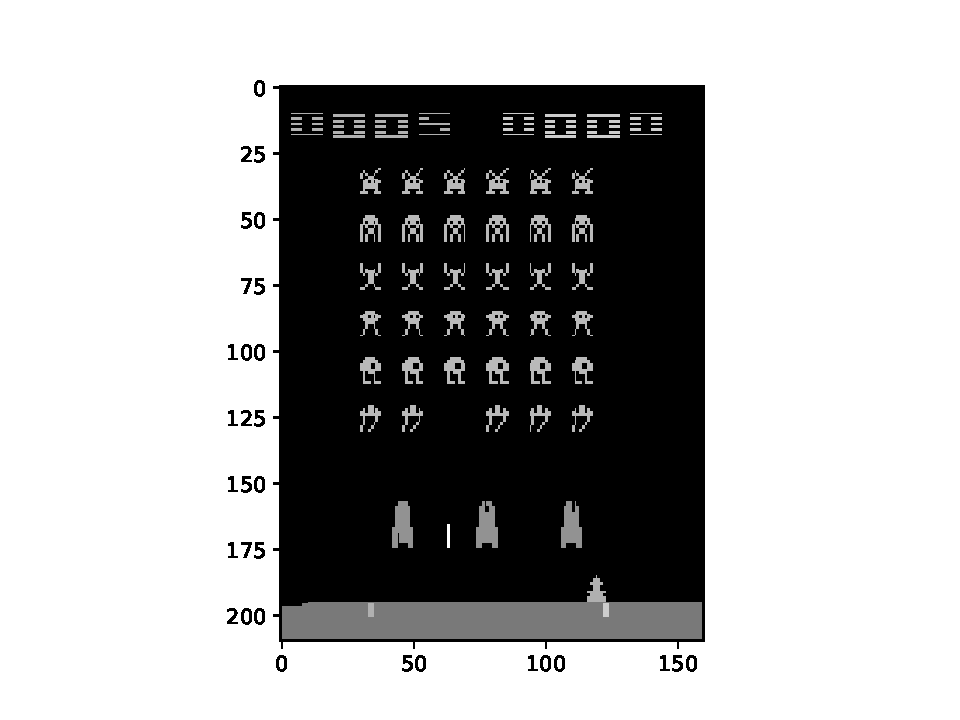
\includegraphics[height=5.8cm]{graphics/atari-pre-processing/3-spaceinvaders-grey-cropped.pdf}
        \caption{}
        \label{fig: Experimental work: atari-pre-processing-3-spaceinvaders-grey}
    \end{subfigure}
    \centering
    \begin{subfigure}[b]{0.40\textwidth}
        \centering
        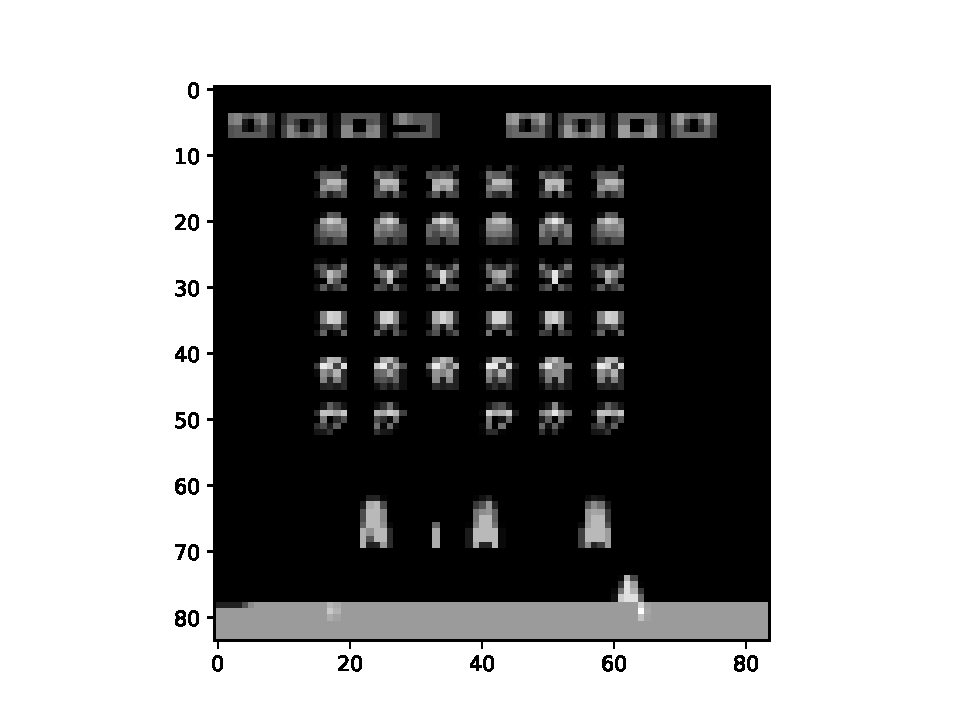
\includegraphics[height=5.8cm]{graphics/atari-pre-processing/4-spaceinvaders-resized-cropped.pdf}
        \caption{}
        \label{fig: Experimental work: atari-pre-processing-4-spaceinvaders-resized}
    \end{subfigure}
    \caption{\subref{fig: Experimental work: atari-pre-processing-1-spaceinvaders-original} Original frame from Space Invaders. \subref{fig: Experimental work: atari-pre-processing-2-spaceinvaders-flicker} Flicker removed by setting pixels to their maximal value over previous four frames. Notice the elongated beam. \subref{fig: Experimental work: atari-pre-processing-3-spaceinvaders-grey} Converted to greyscale. \subref{fig: Experimental work: atari-pre-processing-4-spaceinvaders-resized} Resized to $84\times84$.}
    \label{fig: Experimental work: atari-pre-processing}
\end{figure}

An illustration of the results of this preprocessing can be seen for the game of Space Invaders in \autoref{fig: Experimental work: atari-pre-processing}. Note that the fired beam is longer in \subref{fig: Experimental work: atari-pre-processing-2-spaceinvaders-flicker} compared to \subref{fig: Experimental work: atari-pre-processing-1-spaceinvaders-original}. This is a side effect of combining successive images by pixel maximum which slightly elongates moving objects.

%!TEX root = ../Thesis.tex

\section{Network architectures}\label{sec: Experimental work: Neural network architectures}
%This section describes the \gls{NN} model architectures used for the benchmark problems. Detailed model summaries can be found in \autoref{app: models}.


\subsection{Architecture for MNIST}\label{sec: Experimental work: Neural network architectures (MNIST)}
For the \gls{MNIST} problem, a simple \gls{CNN} with 22.000 parameters has been used. Overall, the network has two convolutional layers each followed by batch normalization, max pooling and a ReLU nonlinearity. Fully connected layers follow; the first with batch normalization and ReLU nonlinearity; the second with log-softmax nonlinearity.

In more detail, the first layer is a convolution layer with $10$ $5\times5$ kernels and $10$ biases and is applied to the single greyscale channel of the input images. This layer is followed by a batch normalization layer with a mean and standard deviation for each of the 10 kernels and a learned affine transformation. A max pooling layer with $2\times2$ kernel and no padding is then applied. Finally, a ReLU nonlinearity is applied. The second convolution layer has $20$ kernels but is otherwise identical to the first also followed by batch normalization, max pooling and ReLU nonlinearity. The following fully connected layer has the $320$ outputs of the preceding convolution layer as input and has $50$ outputs followed by batch normalization and ReLU nonlinearity. The output layer of the model is fully connected with $50$ inputs and $10$ outputs, one for each digit. A log-softmax nonlinearity is applied to the output units and combined with the \gls{NLL} loss. \autoref{lst: Network models: MNIST with batch normalization} contains a summary of this network.


\subsection{Architecture for Atari environments}\label{sec: Experimental work: Neural network architectures (RL}
The network architecture used for learning policies for the Atari environments is the same as the one used by \cite{Mnih2015, Silver2016}. In short, the network is a \gls{CNN} with three convolutional layers followed by two fully connected layers totalling 1.685.667 parameters, most of them in the first linear layer.

In more detail, the first convolutional layer has $32$ $8\times8$ kernels, $32$ biases and is applied to each of the four most recent frames, each of which is treated as a channel. This layer has a stride of $4$ and is followed by a ReLU nonlinearity. The second convolutional layer has $64$ $4\times4$ kernels, $64$ biases and is applied to each of the $32$ $20\times20$ outputs of the previous layer. It has a stride of $2$ and is also followed by a ReLU nonlinearity. The third and final convolutional has $64$ $3\times3$ kernels, $64$ biases and is applied to each of the $64$ $9\times9$ outputs of the previous layer. It has a stride of $1$ and is followed by a ReLU nonlinearity. A fully connected layer with $64\times7\times7=3136$ inputs, $512$ outputs and a ReLU nonlinearity connects the flattened output of the final convolutional layer with the output layer. The output layer is fully connected and followed by a log-softmax nonlinearity with its number of outputs defined by the specific Atari environment. For the Freeway environment it is $3$ while for Seaquest it is $18$. \autoref{lst: Network models: DQN network for Atari environments} contains a summary of this network.



%One for each problem type:
%MNIST
%CIFAR-10 
%- Data set\cite{Krizhevsky2009}
%- Model \cite{Hertel2015}
%Atari



%!TEX root = ../Thesis.tex

\section{Computational scaling}\label{sec: Experimental work: Computational scaling}
%This section presents the parallel scaling capabilities of the \gls{VO} method as applied to both supervised and reinforcement learning problems.

\subsection{Scaling in supervised learning}
\begin{figure}[tbp!]
    \begin{subfigure}[b]{0.517\textwidth}
        \centering
        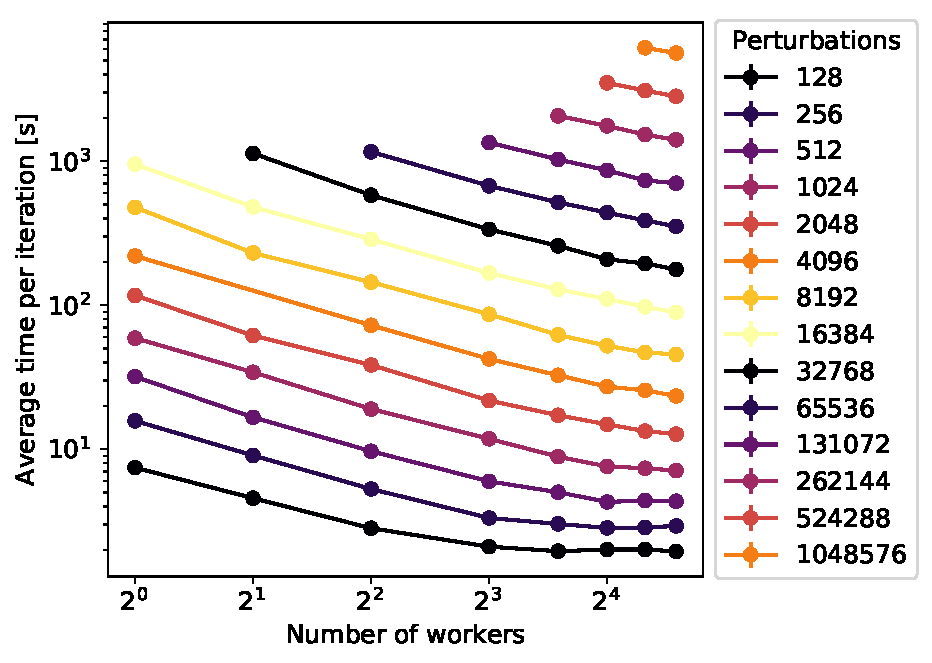
\includegraphics[height=5.6cm]{graphics/E005-sca-analysis/E005-scaling-02.pdf}
        \caption{}
        \label{fig: Theory: E005-scaling-supervised-02}
    \end{subfigure}
    \hfill
    \begin{subfigure}[b]{0.473\textwidth}
        \centering
        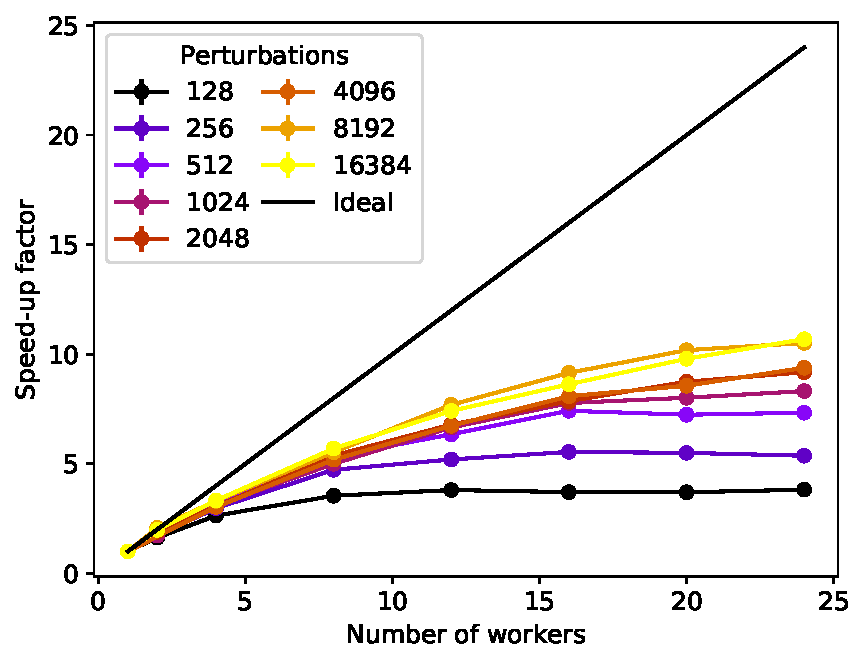
\includegraphics[height=5.6cm]{graphics/E005-sca-analysis/E005-scaling-04.pdf}
        \caption{}
        \label{fig: Theory: E005-scaling-supervised-04}
    \end{subfigure}
    \caption{
        Computational scaling in the supervised setting for different numbers of \glspl{CPU} and perturbations. Each observation is the average over 100 iterations with associated standard deviation (too small to discern).
        \subref{fig: Theory: E005-scaling-supervised-02} The average time spent per iteration in seconds.
        \subref{fig: Theory: E005-scaling-supervised-04} The observed speedup.
    }
    \label{fig: Theory: E005-scaling-supervised}
\end{figure}
This section presents the computational scaling of the \gls{VO} method used to train the \gls{MNIST} architecture described above when using a several \glspl{CPU} and varying the number of perturbations. 
Each setting of number of perturbations was run for 100 iterations and evaluated on a mini-batch of 200 images.
%Each perturbation was evaluated on a mini-batch of 200 images and each iteration of the algorithm evaluates some number of perturbations and was timed. 
The mean time and variance were computed from the 100 iterations run for each combination of number of \glspl{CPU} and perturbations.

\autoref{fig: Theory: E005-scaling-supervised-02} shows the average time spent per iteration as a function of the number of \glspl{CPU} used for various numbers of perturbations. The scaling can be seen to be fairly good for a high enough number of perturbations. Since the evaluation of every perturbation is a single forward pass through the network, the fitness evaluation is quite fast and slower function evaluations would give better scaling. \autoref{fig: Theory: E005-scaling-supervised-04} shows the measured speedup as a function of the number \glspl{CPU} for different perturbations. %This is a popular plot for presenting parallel performance and illustrates Amdahl's law \cite{Amdahl1967}. 
It is evident that speedup quickly drops off from the ideal although an order of magnitude speedup is observed for 24 \glspl{CPU}.

Obviously, \gls{VO} is an inefficient choice for optimizing differentiable \glspl{NN} in the supervised setting. Backpropagation excels at this task while also allowing for efficient batch parallelization on \glspl{GPU}.
%This points out the inefficiency of applying \gls{VO} to cases with relatively low cost fitness evaluations. Higher parallel
%Furthermore, this forward pass can be significantly sped up by using \glspl{GPU}.

\subsection{Scaling on a reinforcement learning problem}
\begin{figure}[tbp!]
    \begin{subfigure}[b]{0.504\textwidth}
        \centering
        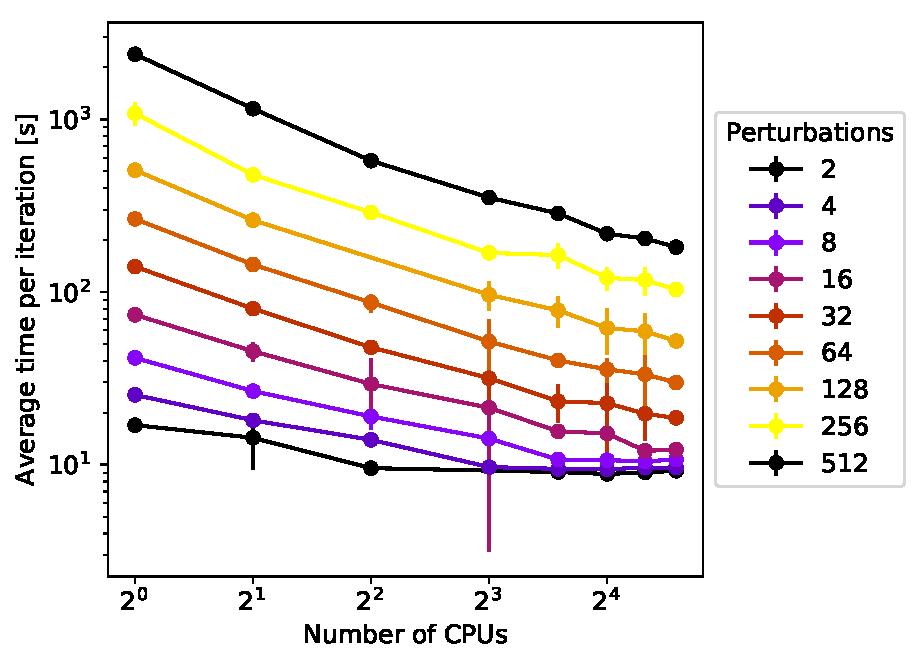
\includegraphics[height=5.7cm]{graphics/E011-sca-analysis/E011-scaling-02.pdf}
        \caption{}
        \label{fig: Theory: E011-scaling-supervised-02}
    \end{subfigure}
    \hfill
    \begin{subfigure}[b]{0.486\textwidth}
        \centering
        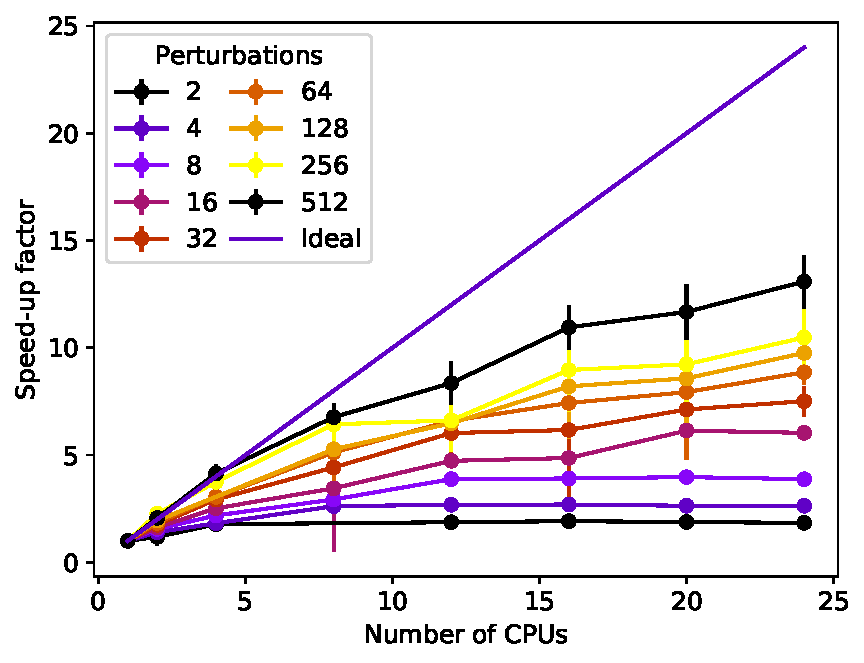
\includegraphics[height=5.7cm]{graphics/E011-sca-analysis/E011-scaling-04.pdf}
        \caption{}
        \label{fig: Theory: E011-scaling-supervised-04}
    \end{subfigure}
    \caption{
        Computational scaling in the reinforcement learning setting for different numbers of \glspl{CPU} and perturbations. Each observation is the average over 100 iterations with associated standard deviation.
        \subref{fig: Theory: E011-scaling-supervised-02} The average time spent per iteration in seconds.
        \subref{fig: Theory: E011-scaling-supervised-04} The observed speedup.
    }
    \label{fig: Theory: E011-scaling-supervised}
\end{figure}

This section presents the results of running the same scaling experiment as before but here on the Atari-2600 game Freeway. The used network is the DQN from \cite{Mnih2015} and preprocessing is as described above. Each episode was limited to 1000 frames (episode horizon) and 100 episodes were simulated for each combination of number of \glspl{CPU} and perturbations. Freeway was chosen since it has a fixed episode duration allowing the use of untrained policies in the experiment. This removes the dependency of the scaling on the quality of the policy.

The results are presented in the same form as for the supervised case in \autoref{fig: Theory: E011-scaling-supervised}. The scaling is somewhat better than for the supervised case and it is achieved for much lower numbers of perturbations as a result of the much more expensive fitness evaluation. For 512 perturbations, increasing the number of \glspl{CPU} from 1 to 4 provides an almost monomial decrease in the time spent per iteration. This is as observed in \cite{Salimans2017} although the computational resources expended for experimentation were much greater than here. Conclusively, reinforcement learning is much more well suited for the \gls{VO} method supervised learning.
%Here, the fitness function evaluation relies on simulation of some often complex environment and the required forward passes of the policy network are inherently sequential.
%!TEX root = ../Thesis.tex


%!TEX root = ../Thesis.tex

\section{Effect of model augmentations and safe mutation}\label{sec: Experimental work: Effects of common model and algorithm augmentations}

\begin{figure}[tbp!]
    \begin{subfigure}[b]{0.49\textwidth}
        \centering
        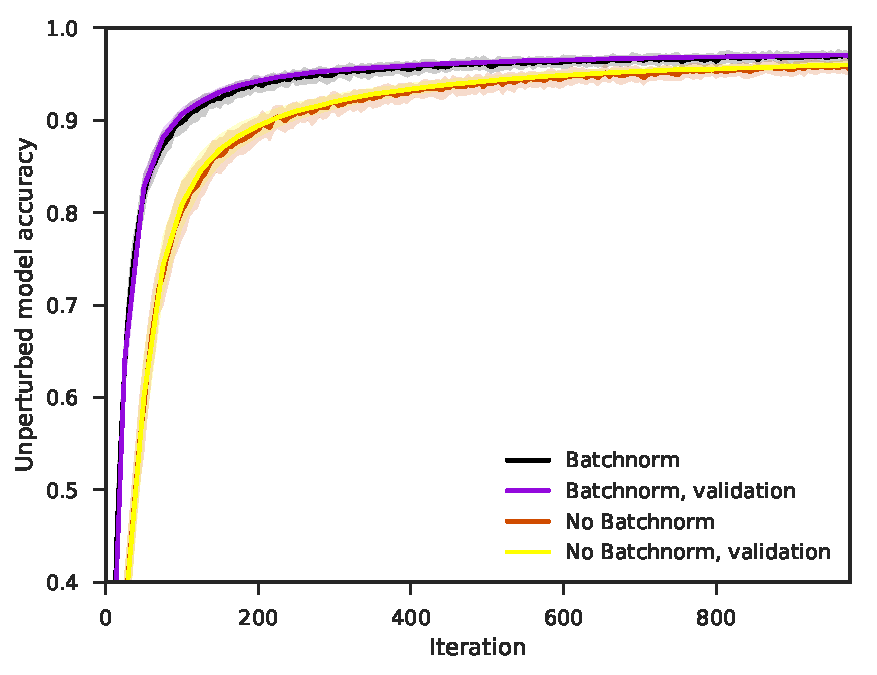
\includegraphics[height=5.8cm]{graphics/E020-bn-analysis/accuracy_unp-all-series-mean-sd.pdf}
        \caption{}
        \label{fig: Theory: E020-bn-analysis/accuracy_unp-all-series-mean-sd}
    \end{subfigure}
    \hfill
    \begin{subfigure}[b]{0.49\textwidth}
        \centering
        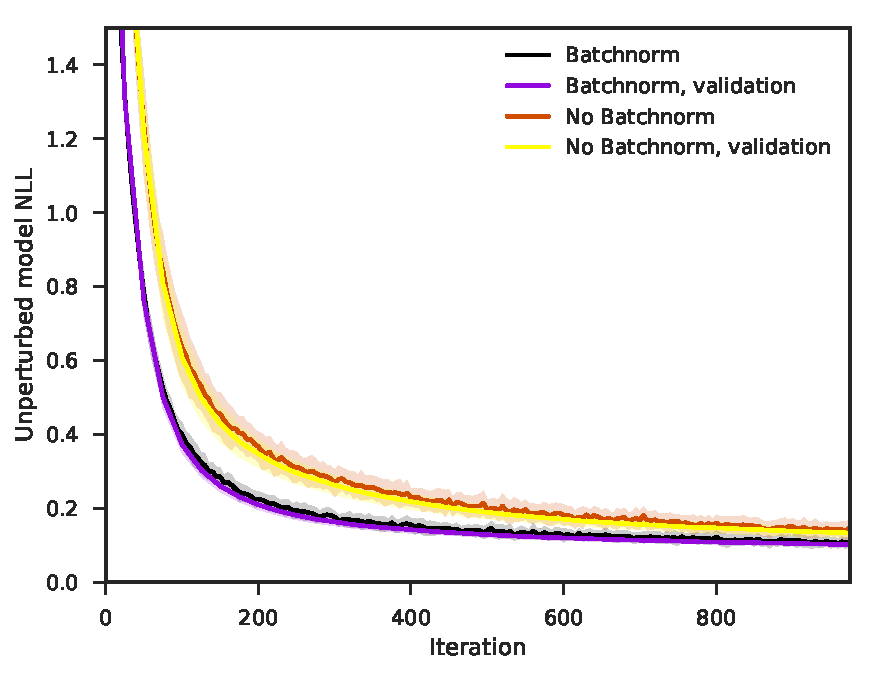
\includegraphics[height=5.8cm]{graphics/E020-bn-analysis/return_unp-all-series-mean-sd.pdf}
        \caption{}
        \label{fig: Theory: E020-bn-analysis/return_unp-all-series-mean-sd}
    \end{subfigure}
    \caption{
        Results of experiments with batch normalization for the unperturbed model.
        \subref{fig: Theory: E020-bn-analysis/accuracy_unp-all-series-mean-sd} Training and validation set classification accuracy.
        \subref{fig: Theory: E020-bn-analysis/return_unp-all-series-mean-sd} Training and validation set \gls{NLL} loss.
        Batch normalization is effective at improving the optimization of the \gls{NN}.
    }
    \label{fig: Theory: E020-bn-analysis}
\end{figure}
This section explores the effects of some common augmentation techniques for \gls{NN} models along with the effects of safe mutation in the \gls{VO} algorithm. The experiments investigate whether the \gls{VO} gradient benefits from the same model improvements as algorithms based on conventional backpropagated gradients do.

The algorithm is isotropic Gaussian \gls{VO} a with fixed variance of $0.05$ similar to \cite{Salimans2017} but uses safe mutation.
%The experiments in this section were performed with the \gls{VO} method listed in \autoref{alg: Canonical variational optimization} using an isotopic Gaussian search distribution but with a fixed $\sigma$ of $0.05$. This algorithm is thus similar to the one used in \cite{Salimans2017} but uses safe mutation.
The experiments were run with 100 perturbations using \gls{SGD} with a momentum of $0.9$ and $L^2$ norm regularization of $0.001$ on all optimized parameters. A learning rate of $0.05$ was used. If nothing else is noted, antithetic sampling and the signed gradient (sum) version of safe mutation were used, batch normalization layers were included in the model and the method of common random numbers was not applied.

The setting is supervised and the data set is \gls{MNIST} for all experiments. The network used is the one for \gls{MNIST} (\autoref{lst: Network models: MNIST with batch normalization}) along with a variant without batch normalization (\autoref{lst: Network models: MNIST without batch normalization}) and a variant without batch normalization and with dropout (\autoref{lst: Network models: MNIST with dropout}).
Each experiment is run for 1000 iterations on mini-batches of 1000 examples for 30 different random seeds. Each experiment shows two plots. The \textbf{(a)} plot shows the classification accuracy for the unperturbed model with each series averaged over the 30 runs at every iteration. The \textbf{(b)} plot shows the \gls{NLL} loss. Both metrics are evaluated on the training set and the test (validation\footnote{The validation set is in fact the remaining part of the data set leaving no data for testing. However, the validation set is not used for fitting any hyperparameters an can as such be regarded a test set as well.}) set during training. The shaded bands indicate one standard deviation among the runs.

Some of these experiments were also run using the Adam optimizer. These plots can be seen in \autoref{app: Effects of common model and algorithm augmentations (Adam optimizer)}. The only difference is the choice of optimizer. The hyperparameter settings for Adam are as recommended in the original paper except for the learning rate which is as for \gls{SGD}. It generally proved to be more difficult to obtain good training characteristics using the Adam optimizer which is hypothesized to be due to the relatively high gradient variance resulting in poor second order moment estimates.


\iffalse
\subsection{Glorot initialization}\label{sec: Experimental work: Glorot initialization}
This section analyzes the results of comparing the default PyTorch initialization scheme with the Glorot initialization scheme \cite{Glorot2010}. \autoref{fig: Theory: E020-init-analysis} shows that initializing the convolutional and linear layers using the Glorot scheme on the \gls{MNIST} network does not yield a signficantly faster learning or better final accuracy compared to the default PyTorch initialization.  In both cases, the learning curves and accuracy curves are almost coincident and within each others standard deviation bands.

That Glorot initialization shows no immediate improvement for the training may here be due to the relatively small network used as well as the simplicity of the problem. Larger networks trained on more challenging data sets may gain more from specialized initialization schemes. Finally, the original paper only applied the scheme to \gls{FNN} without convolutional layers \cite{Glorot2010} which may also influence its effect.

\todo[inline]{WARNING! The default PyTorch initialization is Glorot for linear layers so there really is little difference....}

\begin{figure}[tbp!]
    \begin{subfigure}[b]{0.49\textwidth}
        \centering
        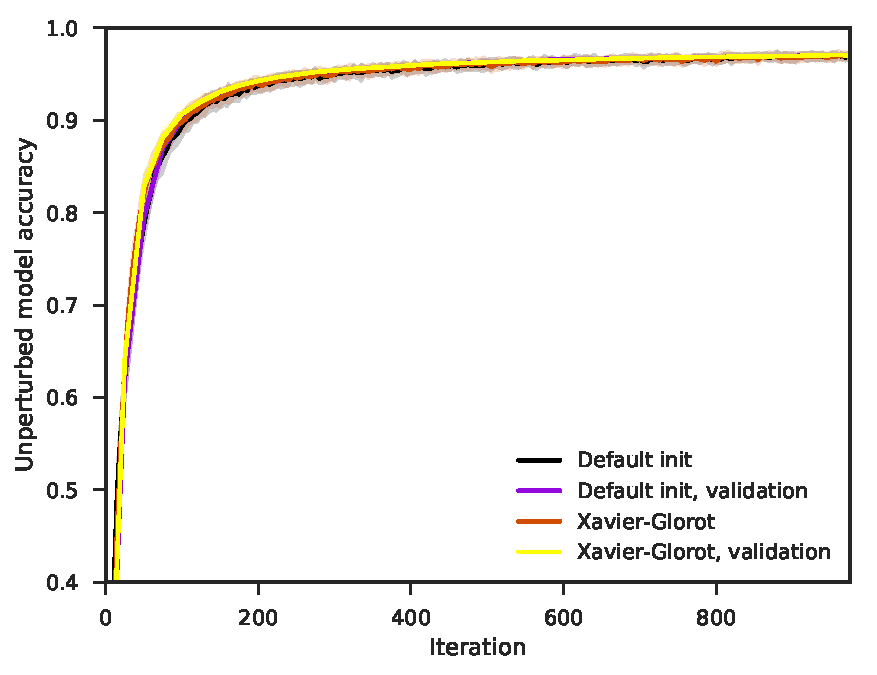
\includegraphics[height=5.8cm]{graphics/E020-init-analysis/accuracy_unp-all-series-mean-sd.pdf}
        \caption{}
        \label{fig: Theory: E020-init-analysis/accuracy_unp-all-series-mean-sd}
    \end{subfigure}
    \hfill
    \begin{subfigure}[b]{0.49\textwidth}
        \centering
        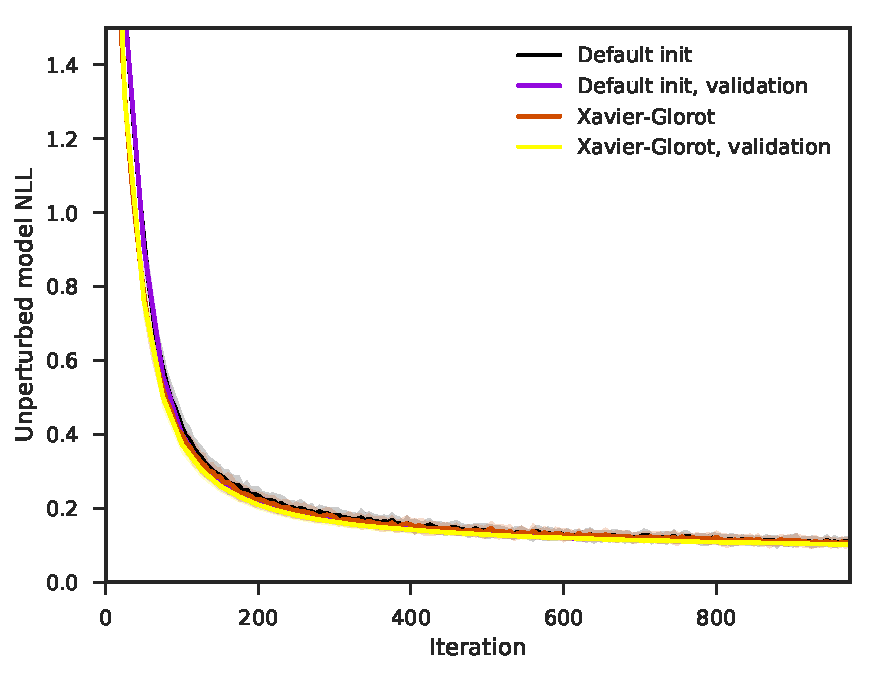
\includegraphics[height=5.8cm]{graphics/E020-init-analysis/return_unp-all-series-mean-sd.pdf}
        \caption{}
        \label{fig: Theory: E020-init-analysis/return_unp-all-series-mean-sd}
    \end{subfigure}
    \caption{
        Results of experiments with initialization scheme for the unperturbed model.
        \subref{fig: Theory: E020-init-analysis/accuracy_unp-all-series-mean-sd} Training and validation set classification accuracy.
        \subref{fig: Theory: E020-init-analysis/return_unp-all-series-mean-sd} Training and validation set \gls{NLL} loss.
    }
    \label{fig: Theory: E020-init-analysis}
\end{figure}
\fi





\subsection{Batch normalization}\label{sec: Experimental work: Batch normalization}
Here, versions of the \gls{MNIST} network with and without batch normalization layers were compared. The positive effect of batch normalization layers between convolution and fully connected layers in the network is evident from \autoref{fig: Theory: E020-bn-analysis}. The network with batch normalization has a significantly steeper loss curve, reaching low losses and high accuracies faster than the network without batch normalization.
It seems the networks asymptote the same final accuracy and loss suggesting that the network without batch normalization is in this case capable of reaching the same level of accuracy as the one with batch normalization, given enough time.
This is in line with the expectated effect of batch normalization as presented in \autoref{chp: Neural networks}. As such, batch normalization can be said to work as expected also with the \gls{VO} gradient which is estimated without the use of backpropagation.



\subsection{Dropout}\label{sec: Experimental work: Dropout}
\begin{figure}[tbp!]
    \begin{subfigure}[b]{0.49\textwidth}
        \centering
        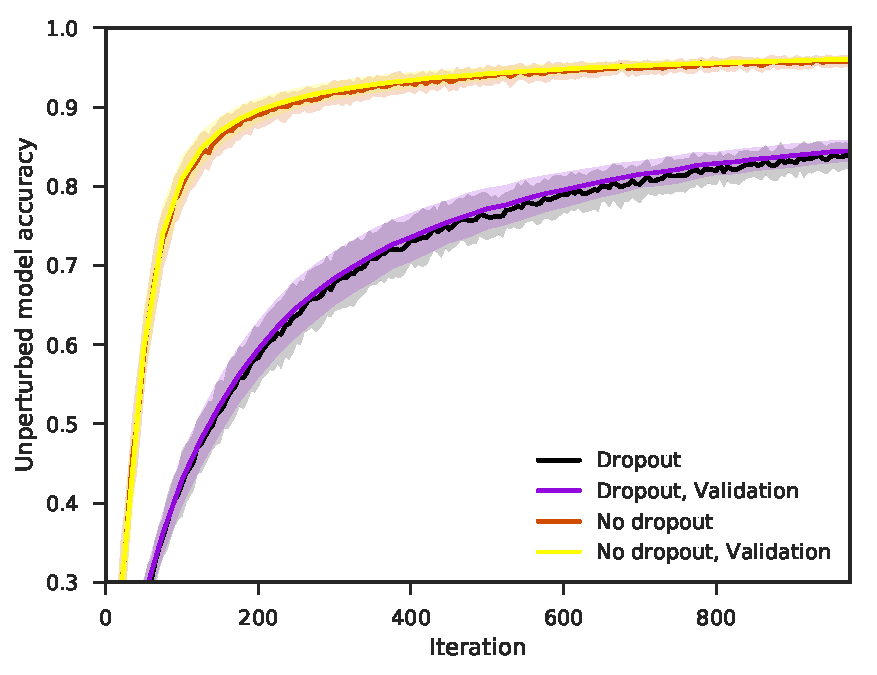
\includegraphics[height=5.8cm]{graphics/E024-DO-SGD-analysis/accuracy_unp-all-series-mean-sd.pdf}
        \caption{}
        \label{fig: Theory: E024-DO-SGD-analysis/accuracy_unp-all-series-mean-sd}
    \end{subfigure}
    \hfill
    \begin{subfigure}[b]{0.49\textwidth}
        \centering
        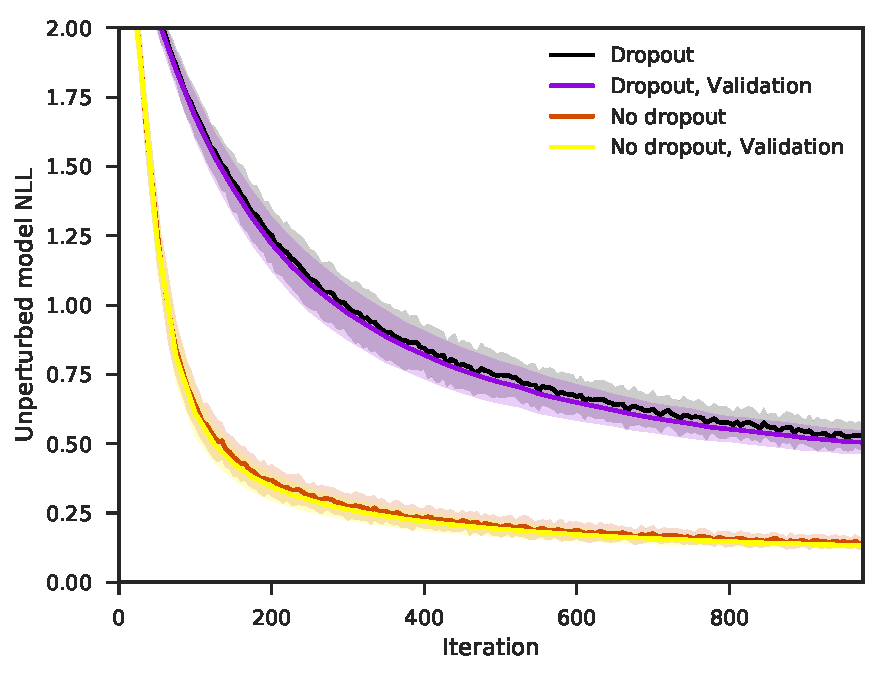
\includegraphics[height=5.8cm]{graphics/E024-DO-SGD-analysis/return_unp-all-series-mean-sd.pdf}
        \caption{}
        \label{fig: Theory: E024-DO-SGD-analysis/return_unp-all-series-mean-sd}
    \end{subfigure}
    \caption{
        Results of experiments with dropout for the unperturbed model.
        \subref{fig: Theory: E024-DO-SGD-analysis/accuracy_unp-all-series-mean-sd} Training and validation set classification accuracy.
        \subref{fig: Theory: E024-DO-SGD-analysis/return_unp-all-series-mean-sd} Training and validation set \gls{NLL} loss. Dropout drastically reduces ease of training probably due to a small network with relatively low capacity and the regularizing effect of optimizing the smoothing \gls{VO} objective.
    }
    \label{fig: Theory: E024-DO-SGD-analysis}
\end{figure}
This section examines the effect of applying dropout to the \gls{MNIST} network. The compared networks are those in \autoref{lst: Network models: MNIST without batch normalization} and \autoref{lst: Network models: MNIST with dropout}, i.e. the network with dropout is compared to a network without dropout. Neither of the networks use batch normalization.

The results of the experiment are shown in \autoref{fig: Theory: E024-DO-SGD-analysis}. The use of dropout results in slower learning and attainment of significantly inferior loss and classification accuracy withing the 1000 iterations. This effect of using dropout is expected to some degree since for the relatively small network used, randomly zeroing weights can drastically reduce model capacity.
Additionally, the \gls{MNIST} network without dropout showed no signs of overfitting in other experiments using the stochastic gradient estimate. As such, dropout was not expected to be able to radically improve performance. 

The fact that no overfitting occurs for this model may be linked to the smoothing of the objective function imposed by using the variational objective. This is most likely a different perspective on the fact that \gls{VO} with a fixed variance optimizes for the average loss of the entire population of perturbations \cite{Lehman2017}. It seems probable that this assists in avoiding overfitting. This observation is also in line with the examples of \autoref{fig: Theory: var-opt-conv-ES-himmelblau}, \ref{fig: Theory: var-opt-conv-VO-R-himmelblau} and \ref{fig: Theory: var-opt-conv-VO-N-himmelblau} where the algorithm with fixed $\sigma$ cannot fully converge on the minimum, and in some sense, thus cannot not overfit it.

\subsection{Safe mutation}
\begin{figure}[tbp!]
    \begin{subfigure}[b]{0.49\textwidth}
        \centering
        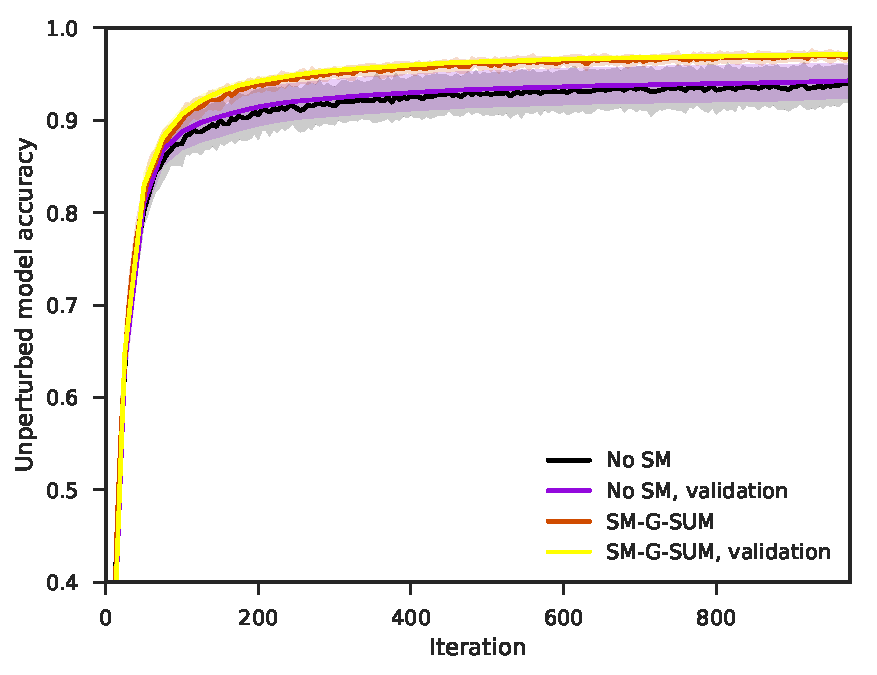
\includegraphics[height=5.8cm]{graphics/E021-SM-analysis/accuracy_unp-all-series-mean-sd.pdf}
        \caption{}
        \label{fig: Theory: E021-SM-analysis/accuracy_unp-all-series-mean-sd}
    \end{subfigure}
    \hfill
    \begin{subfigure}[b]{0.49\textwidth}
        \centering
        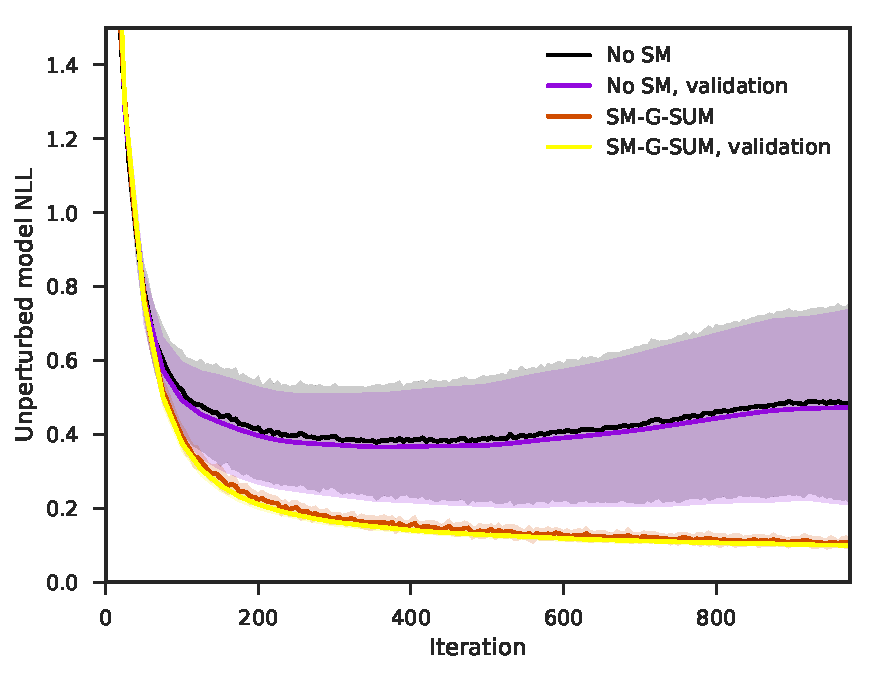
\includegraphics[height=5.8cm]{graphics/E021-SM-analysis/return_unp-all-series-mean-sd.pdf}
        \caption{}
        \label{fig: Theory: E021-SM-analysis/return_unp-all-series-mean-sd}
    \end{subfigure}
    \caption{
        Results of experiments with safe mutation (SM-G-SUM) for the unperturbed model.
        \subref{fig: Theory: E021-SM-analysis/accuracy_unp-all-series-mean-sd} Training and validation set classification accuracy.
        \subref{fig: Theory: E021-SM-analysis/return_unp-all-series-mean-sd} Training and validation set \gls{NLL} loss.
        Scaling perturbations according to network parameter sensitivities results in more stable training.
    }
    \label{fig: Theory: E021-SM-analysis}
\end{figure}
This section compares runs with and without the signed gradient (sum) version of safe mutation \cite{Lehman2017a}.

The results are shown in \autoref{fig: Theory: E021-SM-analysis}. Considering the loss curves, not using safe mutation results in much higher variance among runs with different seeds and yields an over run average loss that is much higher compared to runs using safe mutation. Considering the classification accuracies, the difference between runs with and without safe mutation is smaller although the same trends are observed: Over run variance is higher without safe mutation than it is with and runs without safe mutation reach lower classification accuracies on average. This, along with the high loss, indicates that the variants without safe mutation end up in relatively poor areas of the loss surfaces.

It should be noted that it cannot be ruled out that a lower learning rate exists that allows better performance without safe mutation than what is observed here. For instance, the results presented in \cite{Salimans2017} did not use safe mutation. In this case, the use of safe mutation effectively allows using a higher learning rate which must be expected to result in faster convergence.

\newpage
%!TEX root = ../Thesis.tex

\section{Methods for variance reduction}
This section explores the effects of different variance reduction methods. If nothing else is noted, the training details are as described in \autoref{sec: Experimental work: Effects of common model and algorithm augmentations}.

\subsection{Gradient momentum}\label{sec: Experimental work: Effect of momentum}
Due to the potentially high variance of the \gls{VO} gradient, the use of momentum (see \autoref{sec: Neural networks training: Optimization: SGD with momentum}) can have a positive effect on the convergence speed and training time of \gls{VO}. Three levels of momentum were run for thirty random seeds each. The momentums were $0$, $0.1$ and $0.9$. The results can be seen in \autoref{fig: Theory: E030-MOM-S-analysis}. 
A small benefit can be noted from using a momentum of $0.1$ while using $0.9$ has a large impact on the convergence speed.
It is evident that the \gls{VO} gradient benefits from including momentum.

A momentum of $0.99$ was also included in this experiment but resulted in the algorithm not converging. Instead, the training achieved losses of about $0.6$, oscillating up and down presumably due to the gradient being too dependent on past values to adequately adapt to the loss surface. It is plausible that an optimal value of the momentum for this problem resides somewhere between $0.99$ and $0.1$ but no attempt will be made at finding this value.

When adapting the variance, the effect of momentum on the variance was also examined and found to occasionally be detrimental, especially in the \gls{RL} setting. At times, the gradient associated with the variance would spike at a single iteration, preceded and followed by much smaller gradients. Momentum would then continue to increase the variance for many iterations following the spike resulting in a large variance giving detrimentally large perturbations. Lowering the variance learning rate results in the variance practically not adapting during training. Using dampened momentum aids in suppressing these spikes and is discussed further in \autoref{sec: Experimental work: Effect of adapting the variance}. Alternatively, not using momentum on the variance gradient gives little weight to these spikes and the trend of decreasing variance persists through training as wanted.

\begin{figure}[tbp!]
    \begin{subfigure}[b]{0.49\textwidth}
        \centering
        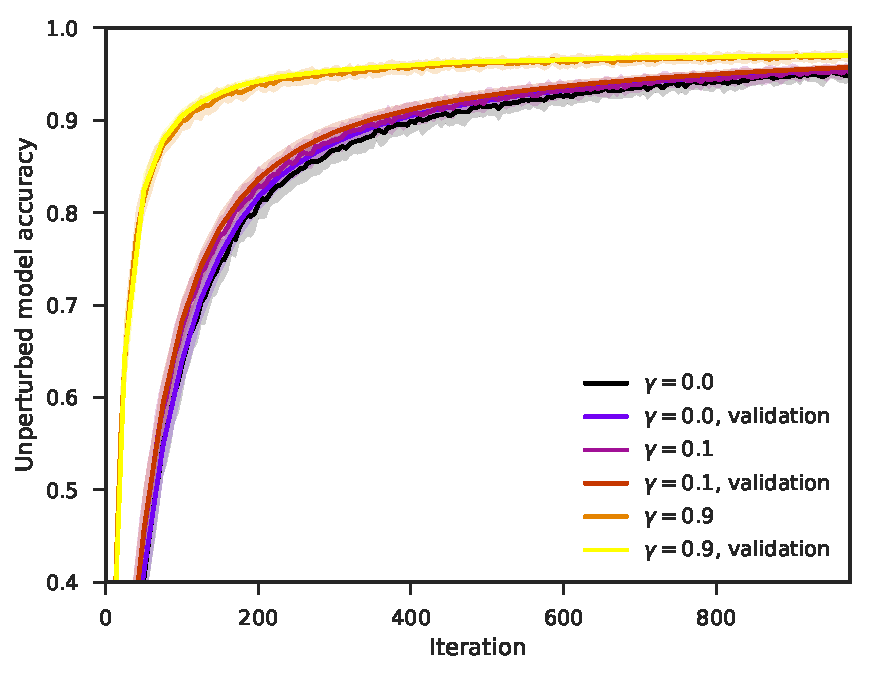
\includegraphics[height=5.8cm]{graphics/E030-MOM-S-analysis/accuracy_unp-all-series-mean-sd.pdf}
        \caption{}
        \label{fig: Theory: E030-MOM-S-analysis/accuracy_unp-all-series-mean-sd}
    \end{subfigure}
    \hfill
    \begin{subfigure}[b]{0.49\textwidth}
        \centering
        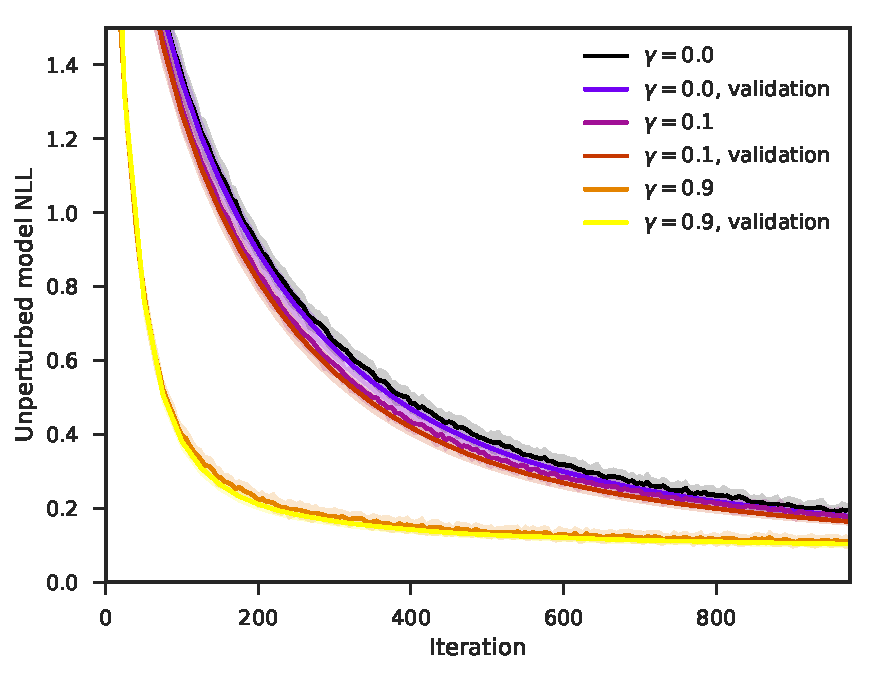
\includegraphics[height=5.8cm]{graphics/E030-MOM-S-analysis/return_unp-all-series-mean-sd.pdf}
        \caption{}
        \label{fig: Theory: E030-MOM-S-analysis/return_unp-all-series-mean-sd}
    \end{subfigure}
    \caption{
        Results of experiments using \gls{SGD} with momentum on the \gls{VO} gradient for the unperturbed model run on \gls{MNIST}.
        \subref{fig: Theory: E030-MOM-S-analysis/accuracy_unp-all-series-mean-sd} Training and validation set classification accuracy.
        \subref{fig: Theory: E030-MOM-S-analysis/return_unp-all-series-mean-sd} Training and validation set \gls{NLL} loss.
        Gradient momentum is effective at reducing the gradient variance and results in faster convergence.
    }
    \label{fig: Theory: E030-MOM-S-analysis}
\end{figure}


\subsection{Antithetic sampling}\label{sec: Experimental work: Antithetic sampling}
In this section, the improvement by using antithetic sampling is experimentally validated. The \gls{MNIST} network was trained using 100 perturbations with antithetic sampling (50 unique, 50 mirrored), 100 perturbations without antithetic sampling and 50 perturbations without antithetic sampling. 

The runs using 100 perturbations with antithetic sampling compares to the runs using 100 perturbations without antithetic sampling in the way that both estimate the gradient from 100 perturbations. From this comparison it can be assessed whether the antithetic samples carry more information than the regular uninformed samples.

The grounds for comparison of runs using 50 perturbations without and 100 perturbations with antithetic sampling is that both of these versions perturb an 50-dimensional subspace of the network parameter space at every iteration of \glsfirst{VO}.
Additionally, the computational complexity of sampling is half as high when using antithetic sampling.
Obviously, the time complexity of the sampling operation is negligible compared to the fitness evaluation so comparison in this basis is not entirely fair.

The results are shown in \autoref{fig: Theory: E022-AS-analysis}. It is evident that using antithetic sampling results in a significant improvement when comparing to both runs with 50 and 100 perturbations. As opposed to the effect seen when including batch normalization, the loss curves initially rise with approximately the same slope but do not asymptote the same value. Thus, the benefit from using antithetic sampling is not faster training but rather the location of a better local minimum and thus better final performance. This is almost certainly due to a reduction in the gradient estimate variance. 

\begin{figure}[tbp!]
    \begin{subfigure}[b]{0.49\textwidth}
        \centering
        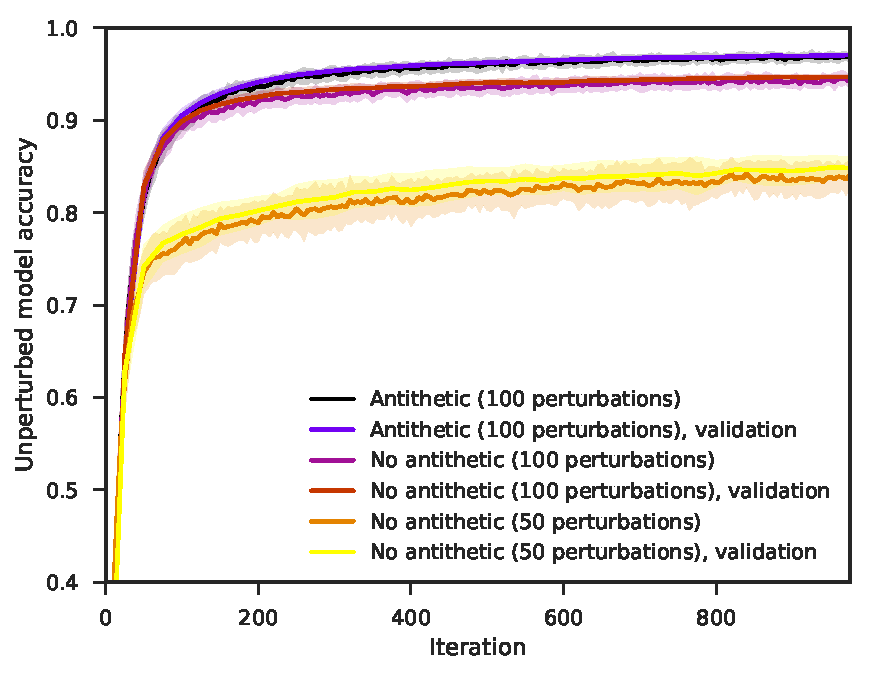
\includegraphics[height=5.8cm]{graphics/E022-AS-analysis/accuracy_unp-all-series-mean-sd.pdf}
        \caption{}
        \label{fig: Theory: E022-AS-analysis/accuracy_unp-all-series-mean-sd}
    \end{subfigure}
    \hfill
    \begin{subfigure}[b]{0.49\textwidth}
        \centering
        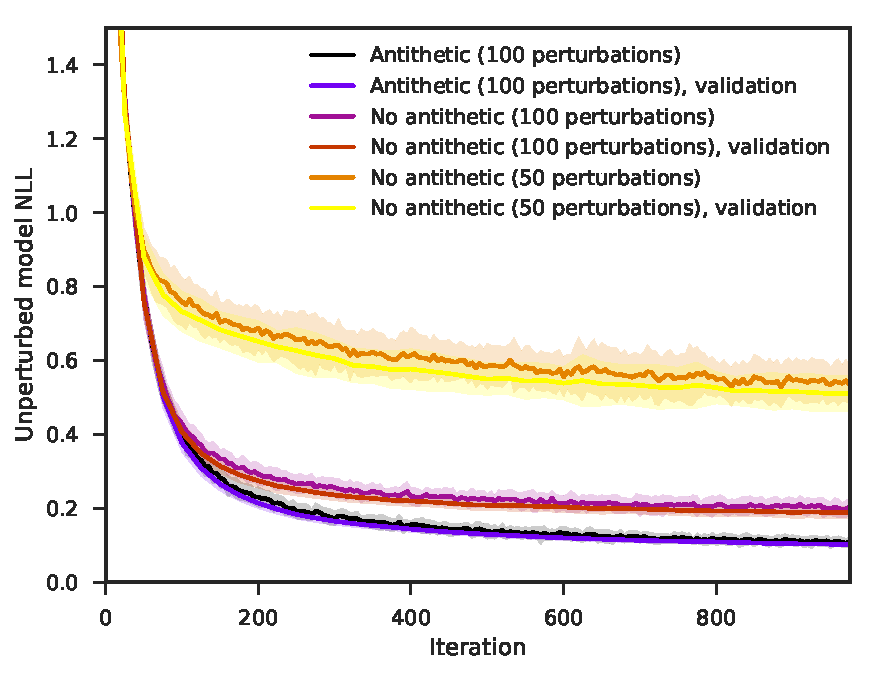
\includegraphics[height=5.8cm]{graphics/E022-AS-analysis/return_unp-all-series-mean-sd.pdf}
        \caption{}
        \label{fig: Theory: E022-AS-analysis/return_unp-all-series-mean-sd}
    \end{subfigure}
    \caption{
        Results of experiments with antithetic sampling for the unperturbed model.
        \subref{fig: Theory: E022-AS-analysis/accuracy_unp-all-series-mean-sd} Training and validation set classification accuracy.
        \subref{fig: Theory: E022-AS-analysis/return_unp-all-series-mean-sd} Training and validation set \gls{NLL} loss.
    }
    \label{fig: Theory: E022-AS-analysis}
\end{figure}

\subsection{Importance mixing}
This section presents results of using importance mixing. This comparison is made in spite of the importance weight collapse and the numerical problems associated with it. In practice some weights become infinite which leads to some reuse of some perturbations. 

\autoref{fig: Theory: E025-IS-analysis} compares a run with importance mixing $(\alpha=0.01)$ and a run without $(\alpha=1.0)$. The \gls{NLL} when using importance mixing is slightly higher than when not. This observation is present in the resulting classification accuracy as well. This detrimental effect must be concluded to stem from the collapse of the importance weights as previously discussed.

\begin{figure}[tbp!]
    \begin{subfigure}[b]{0.49\textwidth}
        \centering
        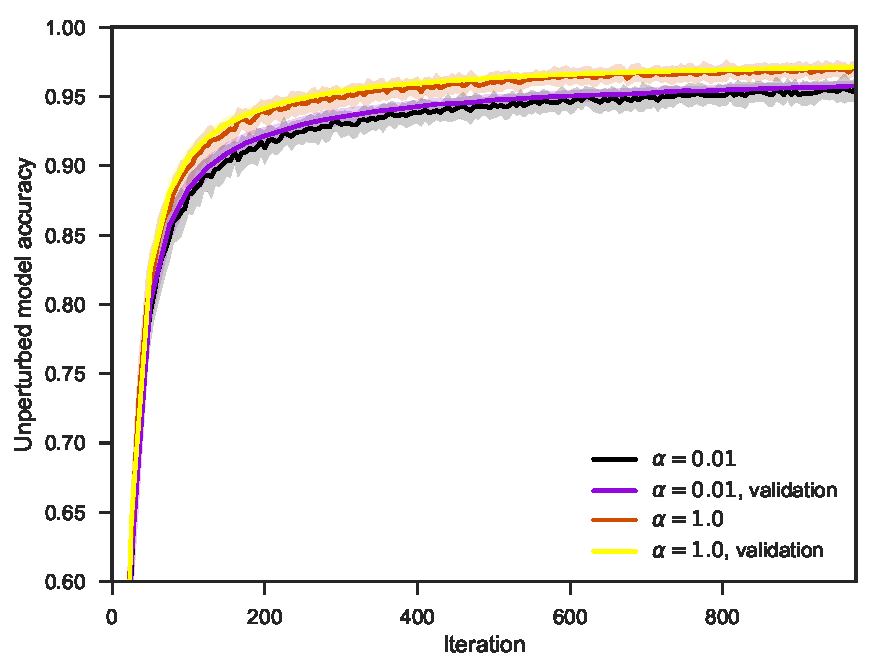
\includegraphics[height=5.8cm]{graphics/E025-IS-analysis/accuracy_unp-all-series-mean-sd.pdf}
        \caption{}
        \label{fig: Theory: E025-IS-analysis/accuracy_unp-all-series-mean-sd}
    \end{subfigure}
    \hfill
    \begin{subfigure}[b]{0.49\textwidth}
        \centering
        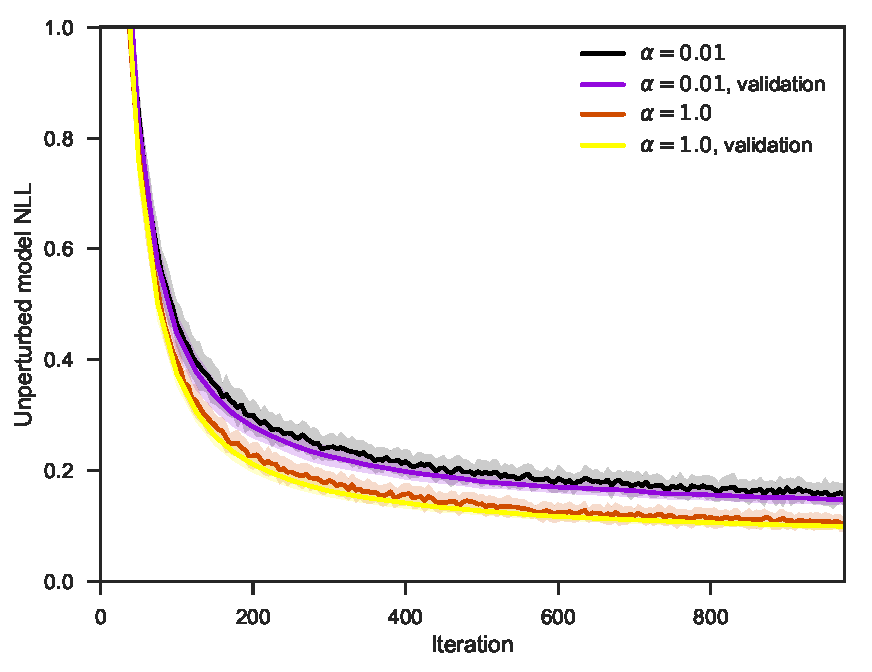
\includegraphics[height=5.8cm]{graphics/E025-IS-analysis/return_unp-all-series-mean-sd.pdf}
        \caption{}
        \label{fig: Theory: E025-IS-analysis/return_unp-all-series-mean-sd}
    \end{subfigure}
    \caption{
        Results of experiments with importance mixing for the unperturbed model.
        \subref{fig: Theory: E025-IS-analysis/accuracy_unp-all-series-mean-sd} Training and validation set classification accuracy.
        \subref{fig: Theory: E025-IS-analysis/return_unp-all-series-mean-sd} Training and validation set \gls{NLL} loss.
    }
    \label{fig: Theory: E025-IS-analysis}
\end{figure}

For comparison, \autoref{fig: Theory: E026-IS-analysis} presents results runs where importance mixing has been replaced by random reuse of perturbations. In the runs with importance mixing, about 10 of the 100 perturbations where effectively reused at each iteration. Therefore, the experiment with random reuse reused 10 perturbations randomly at each iteration. It can be observed that the effect of randomly reusing perturbations is smaller than that of importance mixing, although it remains detrimental compared to reusing no perturbations.

\begin{figure}[tbp!]
    \begin{subfigure}[b]{0.49\textwidth}
        \centering
        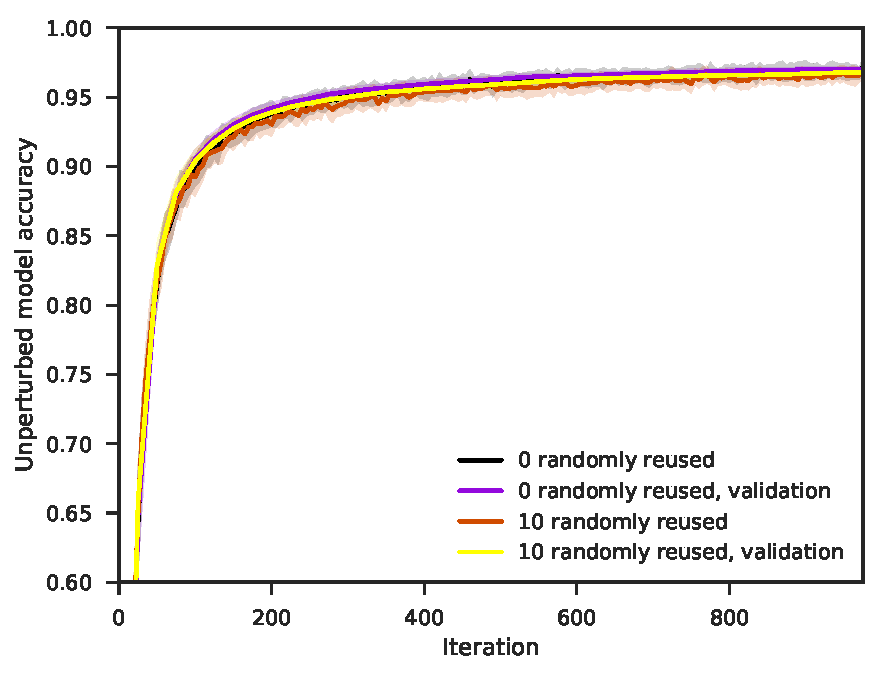
\includegraphics[height=5.8cm]{graphics/E026-IS-analysis/accuracy_unp-all-series-mean-sd.pdf}
        \caption{}
        \label{fig: Theory: E026-IS-analysis/accuracy_unp-all-series-mean-sd}
    \end{subfigure}
    \hfill
    \begin{subfigure}[b]{0.49\textwidth}
        \centering
        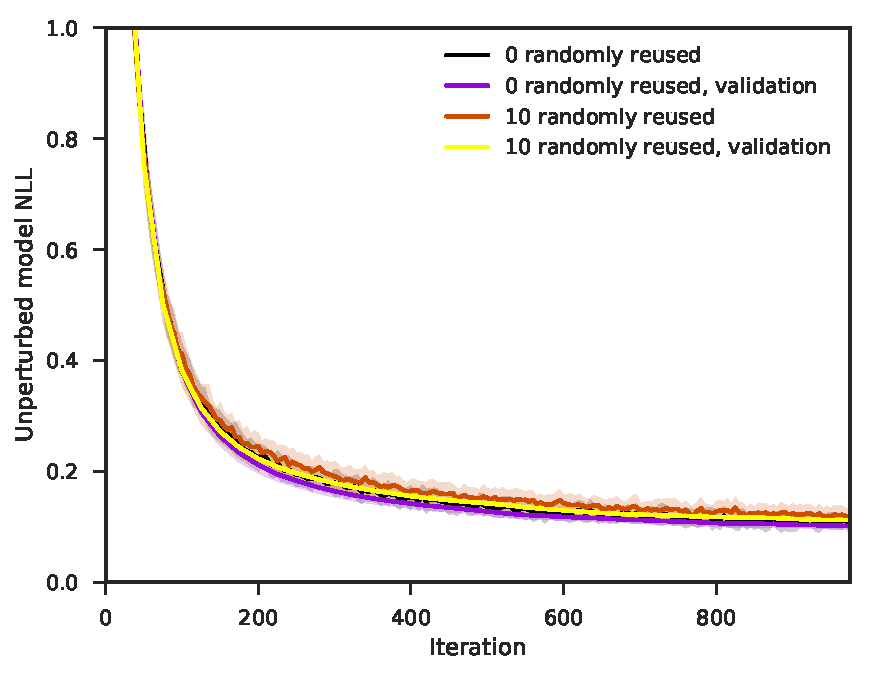
\includegraphics[height=5.8cm]{graphics/E026-IS-analysis/return_unp-all-series-mean-sd.pdf}
        \caption{}
        \label{fig: Theory: E026-IS-analysis/return_unp-all-series-mean-sd}
    \end{subfigure}
    \caption{
        Results of experiments with random resampling for the unperturbed model.
        \subref{fig: Theory: E026-IS-analysis/accuracy_unp-all-series-mean-sd} Training and validation set classification accuracy.
        \subref{fig: Theory: E026-IS-analysis/return_unp-all-series-mean-sd} Training and validation set \gls{NLL} loss.
    }
    \label{fig: Theory: E026-IS-analysis}
\end{figure}

One can note that randomly reusing perturbations is likely to break to assumption that the set of perturbations follows the search distribution, i.e. the Gaussian in this case. Since the gradient estimators rely on this assumption, the detrimental effect of random reuse of perturbations is expected. Importance mixing is designed to maintain the distribution of the perturbations but due to the collapse of the importance weights this is not the case in practice.






% \subsection{Adaptation sampling}
% \todo[inline]{Run the experiment on using adaptation sampling on \gls{MNIST} model}
% \todo[inline]{Discuss experimental results of adaptation sampling}





\subsection{Common random numbers}
This section presents results using the method of \gls{CRN}. The \gls{MNIST} network was trained using 100 perturbations with and without \gls{CRN} resulting in the training curves illustrated in \autoref{fig: Theory: E027-CRN-S-analysis}. \gls{CRN} was also tested in the \gls{RL} setting with resulting learning curves seen in \autoref{fig: Theory: E028-CRN-R-analysis}. The \gls{RL} runs were made using 40 perturbations for computational feasibility.

There is a small and almost insignificant benefit to using \gls{CRN} in the case of supervised learning on \gls{MNIST}. It can be seen that using \gls{CRN}, the training and validation accuracy and loss slightly outperform those of runs that did not use \gls{CRN} on average but within one standard deviation.

The method was also tested in the \gls{RL} setting with $45$ episodes simulated for each of the shared and random seeds versions.
The results are seen for Freeway in \autoref{fig: Theory: E028-CRN-R1-analysis/return_unp-all-series-mean-sd} and  Seaquest in \autoref{fig: Theory: E028-CRN-R2-analysis/return_unp-all-series-mean-sd}. The average population reward is plotted versus iteration number. 
The picture is similar to that of supervised learning with no significant improvement to be seen by using shared seeds for the simulations. 
As such, the method of \gls{CRN} cannot be concluded to improve on the \gls{VO} gradient estimate.

\begin{figure}[tbp!]
    \begin{subfigure}[b]{0.49\textwidth}
        \centering
        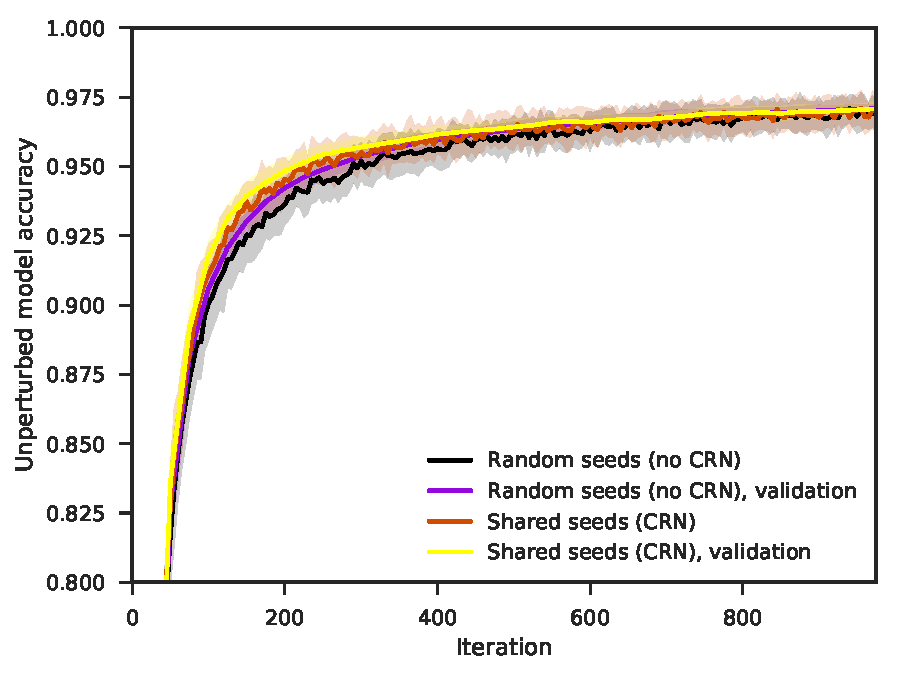
\includegraphics[height=5.7cm]{graphics/E027-CRN-S-analysis/accuracy_unp-all-series-mean-sd.pdf}
        \caption{}
        \label{fig: Theory: E027-CRN-S-analysis/accuracy_unp-all-series-mean-sd}
    \end{subfigure}
    \hfill
    \begin{subfigure}[b]{0.49\textwidth}
        \centering
        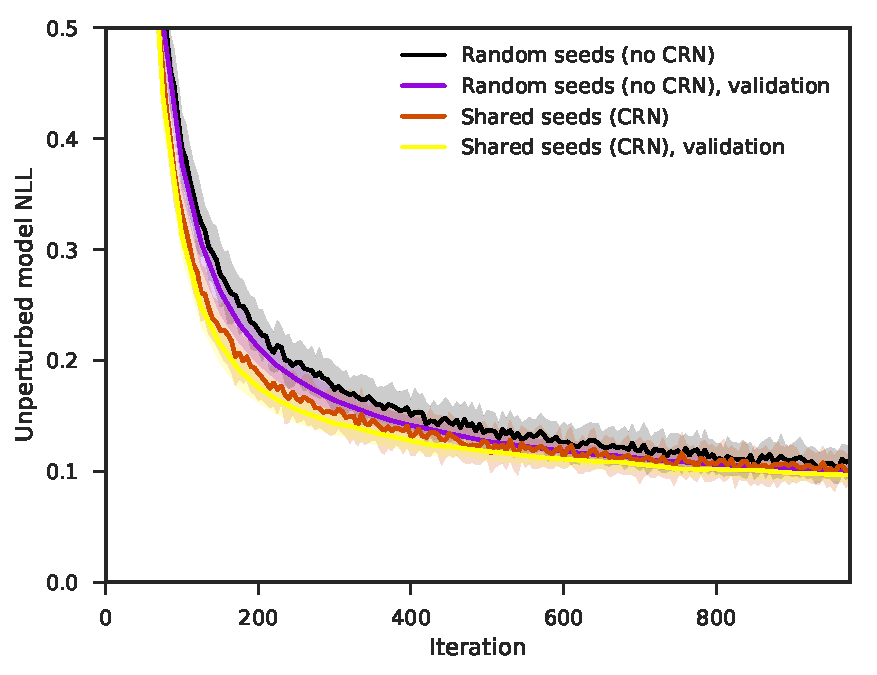
\includegraphics[height=5.7cm]{graphics/E027-CRN-S-analysis/return_unp-all-series-mean-sd.pdf}
        \caption{}
        \label{fig: Theory: E027-CRN-S-analysis/return_unp-all-series-mean-sd}
    \end{subfigure}
    \caption{
        Results of experiments with \glsfirst{CRN} for the unperturbed model run on \gls{MNIST}.
        \subref{fig: Theory: E027-CRN-S-analysis/accuracy_unp-all-series-mean-sd} Training and validation set classification accuracy.
        \subref{fig: Theory: E027-CRN-S-analysis/return_unp-all-series-mean-sd} Training and validation set \gls{NLL} loss.
    }
    \label{fig: Theory: E027-CRN-S-analysis}
\end{figure}
\begin{figure}[tbp!]
    \begin{subfigure}[b]{0.49\textwidth}
        \centering
        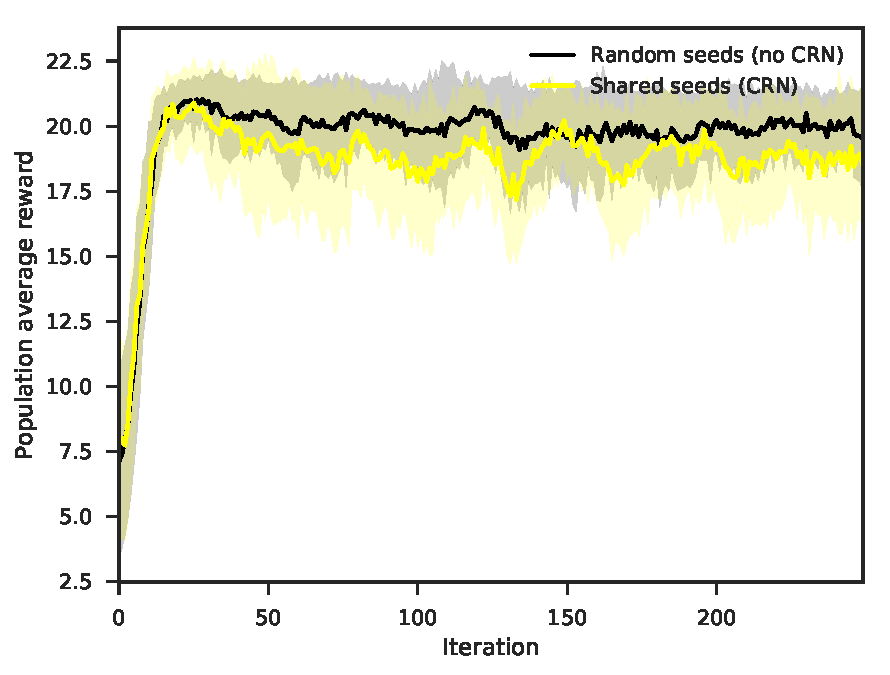
\includegraphics[height=5.8cm]{graphics/E028-CRN-R1-analysis/return_avg-all-series-mean-sd.pdf}
        \caption{}
        \label{fig: Theory: E028-CRN-R1-analysis/return_unp-all-series-mean-sd}
    \end{subfigure}
    \hfill
    \begin{subfigure}[b]{0.49\textwidth}
        \centering
        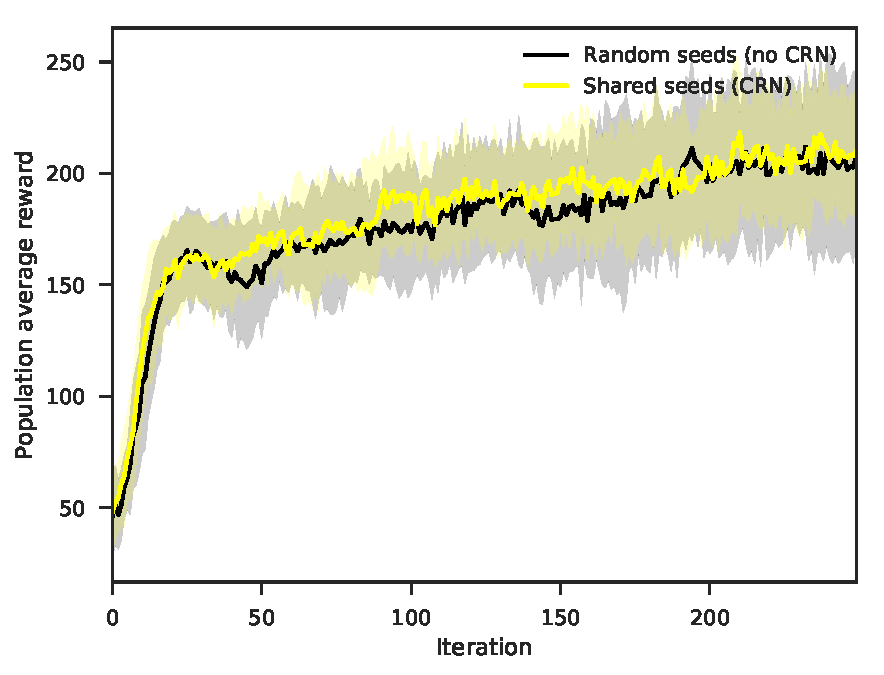
\includegraphics[height=5.8cm]{graphics/E028-CRN-R2-analysis/return_avg-all-series-mean-sd.pdf}
        \caption{}
        \label{fig: Theory: E028-CRN-R2-analysis/return_unp-all-series-mean-sd}
    \end{subfigure}
    \caption{
        Results of experiments with \glsfirst{CRN} for the population average on \subref{fig: Theory: E028-CRN-R1-analysis/return_unp-all-series-mean-sd} Freeway and \subref{fig: Theory: E028-CRN-R2-analysis/return_unp-all-series-mean-sd} Seaquest. The average reward of the population is plotted as a function of \gls{VO} iterations.
    }
    \label{fig: Theory: E028-CRN-R-analysis}
\end{figure}



%!TEX root = ../Thesis.tex

\section{Effect of adapting the variance}\label{sec: Experimental work: Effect of adapting the variance}
Until now, all experiments have been run with an isotropic Gaussian with fixed variance similarly to \cite{Salimans2017}. Here, different variants of the Gaussian search distribution with adaptive variance will be examined.
The examined variants are the isotropic Gaussian, the layer-wise separable Gaussian and the parameter-wise separable Gaussian. For the layer-wise separable Gaussian, a single variance parameter is used for each weight/kernel matrix and bias vector in the model.
Hyperparameters are otherwise as in \autoref{sec: Experimental work: Effects of common model and algorithm augmentations}.

For these experiments, a momentum of $0.9$ has been used on the parameter gradient as well as the adapted variance gradient while the variance gradient is also dampened by $0.9$. Dampening the variance gradient makes sure it does not spike as discussed in \autoref{sec: Experimental work: Effect of momentum}. Dampened momentum on the variance gradient results in much smoother updates to the variance than applying no momentum or non-dampened momentum. Learning rates of $2$ and $4$ have been used for the isotropic and separable Gaussian variances, respectively.


\subsection{Adapting the variance}
\autoref{fig: Theory: E029-VO-S5-MD-analysis} shows the results of running the \gls{VO} algorithm on the MNIST network with the different search distributions. 
\autoref{fig: Theory: E029-VO-S5-MD-analysis/accuracy_val-all-series-mean-sd} and \ref{fig: Theory: E029-VO-S5-MD-analysis/return_val-all-series-mean-sd} respectively show the validation set accuracy and \gls{NLL} loss for the different search distributions.
The most notable difference between the variations is that when the variance is adapted, the isotropic Gaussian gives somewhat unstable learning, in that it gives quite different results solely dependent on random seed.
This can be seen not to be the case when adapting a layer- or parameter-wise separable Gaussians. 

Despite this, the convergence rate and the median final \gls{NLL} loss and accuracy are not improved when using these adaptive search distributions compared to using the fixed isotropic Gaussian. 
Considering the single best and worst performing models on the validation set, it can be noted that these are all obtained by the separable versions. As such, adapting the variance seems to encourage more extensive exploration of the loss landscape but with risk of landing in both a slightly better and slightly worse minimum than would have been reached with a fixed variance.

It should be noted that these observations hold for many different learning rates for the variance parameter(s).

\begin{figure}[tbp!]
    \begin{subfigure}[b]{0.49\textwidth}
        \centering
        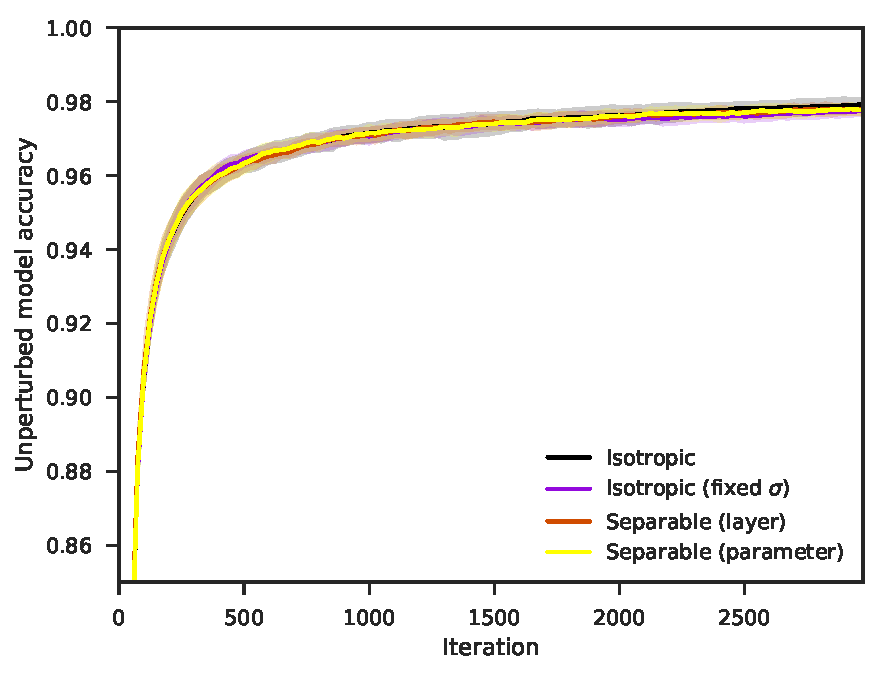
\includegraphics[height=5.8cm]{graphics/E029-VO-S5-MD-analysis/accuracy_val-all-series-mean-sd.pdf}
        \caption{}
        \label{fig: Theory: E029-VO-S5-MD-analysis/accuracy_val-all-series-mean-sd}
    \end{subfigure}
    \hfill
    \begin{subfigure}[b]{0.49\textwidth}
        \centering
        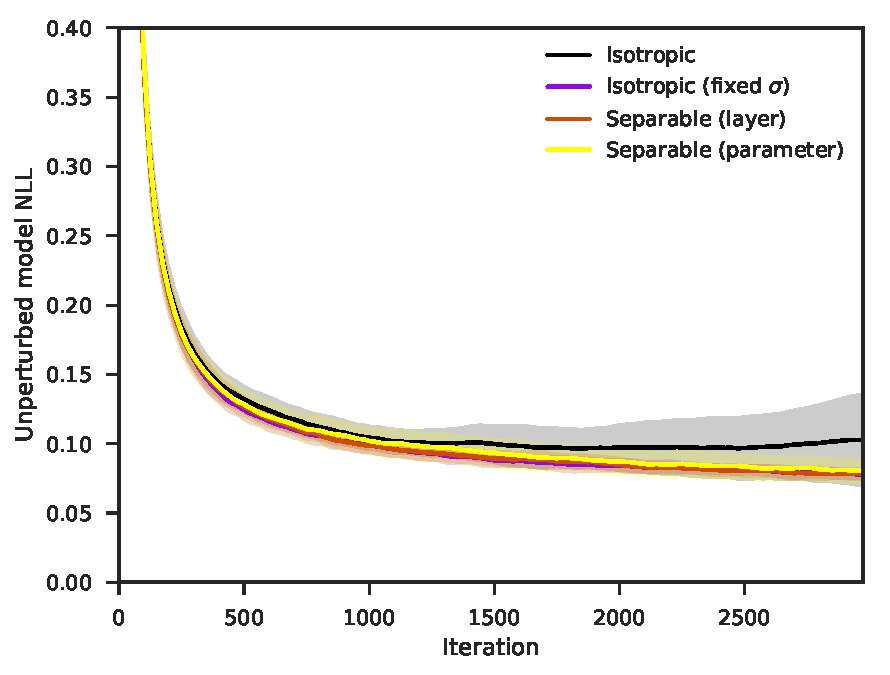
\includegraphics[height=5.8cm]{graphics/E029-VO-S5-MD-analysis/return_val-all-series-mean-sd.pdf}
        \caption{}
        \label{fig: Theory: E029-VO-S5-MD-analysis/return_val-all-series-mean-sd}
    \end{subfigure}
    \begin{subfigure}[b]{0.49\textwidth}
        \centering
        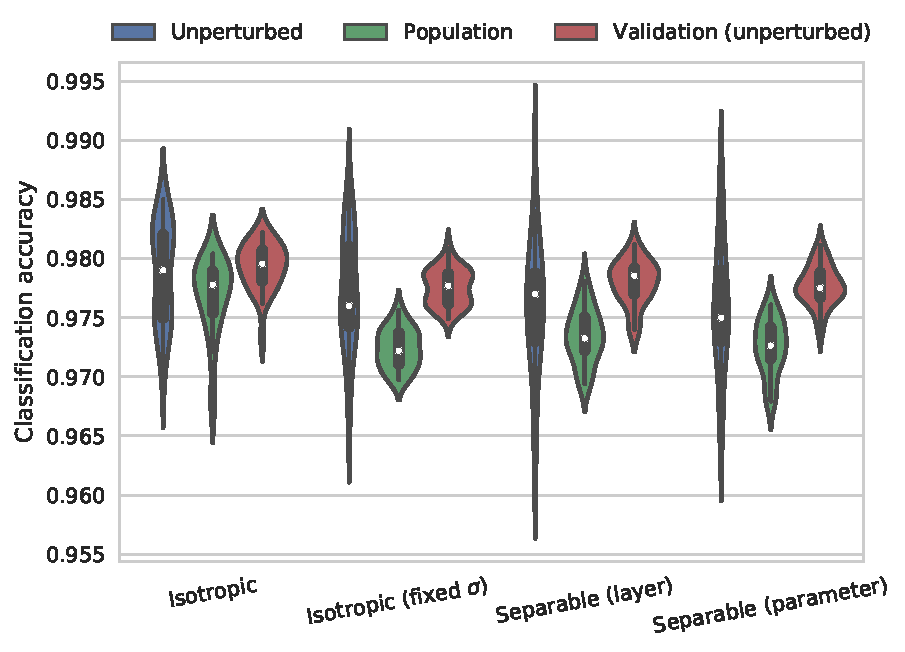
\includegraphics[height=5.3cm]{graphics/E029-VO-S5-MD-analysis/accuracy-final-distribution-boxplot-grouped.pdf}
        \caption{}
        \label{fig: Theory: E029-VO-S5-MD-analysis/accuracy-final-distribution-boxplot-grouped}
    \end{subfigure}
    \hfill
    \begin{subfigure}[b]{0.49\textwidth}
        \centering
        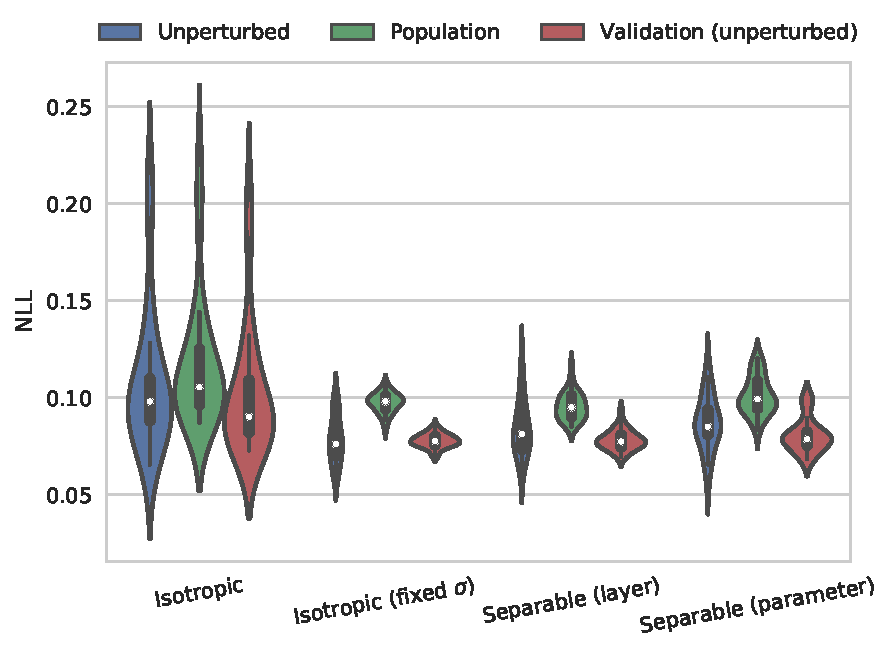
\includegraphics[height=5.3cm]{graphics/E029-VO-S5-MD-analysis/return-final-distribution-boxplot-grouped.pdf}
        \caption{}
        \label{fig: Theory: E029-VO-S5-MD-analysis/return-final-distribution-boxplot-grouped}
    \end{subfigure}
    \caption{
        Results of experiments with different \gls{VO} algorithms. The model variations are the fixed variance strategy of \cite{Salimans2017} and \gls{VO} with adjusted variance using an isotropic Gaussian and respectively a layer-wise and per-weight separable Gaussian. Contrary to \cite{Salimans2017}, safe mutation is applied.
        Plotted versus the iteration number, \subref{fig: Theory: E029-VO-S5-MD-analysis/accuracy_val-all-series-mean-sd} shows the validation set classification accuracy and \subref{fig: Theory: E029-VO-S5-MD-analysis/return_val-all-series-mean-sd} the validation set \gls{NLL} loss. 
        Difference in performance between the algorithms is very small and within one standard deviation with the adapted isotropic having high between-run variance.
        In \subref{fig: Theory: E029-VO-S5-MD-analysis/accuracy-final-distribution-boxplot-grouped} and \subref{fig: Theory: E029-VO-S5-MD-analysis/return-final-distribution-boxplot-grouped} the final distribution of the classification accuracy and \gls{NLL} loss from \subref{fig: Theory: E029-VO-S5-MD-analysis/accuracy_val-all-series-mean-sd} and \subref{fig: Theory: E029-VO-S5-MD-analysis/return_val-all-series-mean-sd} are shown. It can be noted that adapting the variance in the isotropic Gaussian search distribution results a much wider span of the final \gls{NLL} loss. Additionally, a small group of runs has an even higher final \gls{NLL} loss than the main body of runs. This is not observed for the other versions.
        %These seem to hint at a potential better final performance by adapting the variance of a layer-wise separable Gaussian search distribution.
        %which is more flexible than an isotropic Gaussian but has fewer parameters and is easier to estimate than a separable Gaussian with per-weight variances.
    }
    \label{fig: Theory: E029-VO-S5-MD-analysis}
\end{figure}


% \begin{figure}[tbp!]
%     \begin{subfigure}[b]{0.49\textwidth}
%         \centering
%         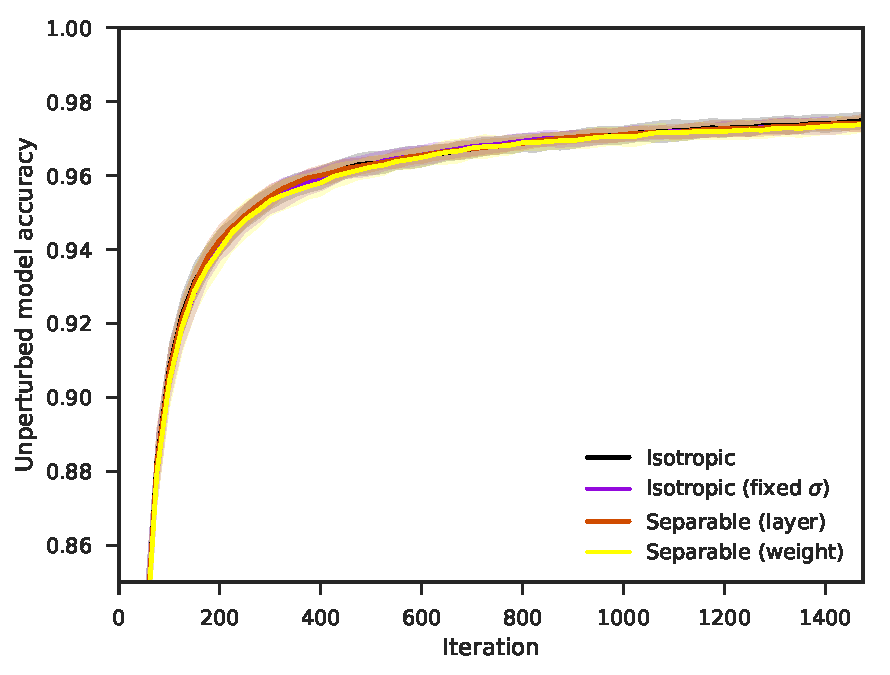
\includegraphics[height=5.8cm]{graphics/E029-VO-S3-analysis-1500/accuracy_val-all-series-mean-sd.pdf}
%         \caption{}
%         \label{fig: Theory: E029-VO-S3-analysis-1500/accuracy_val-all-series-mean-sd}
%     \end{subfigure}
%     \hfill
%     \begin{subfigure}[b]{0.49\textwidth}
%         \centering
%         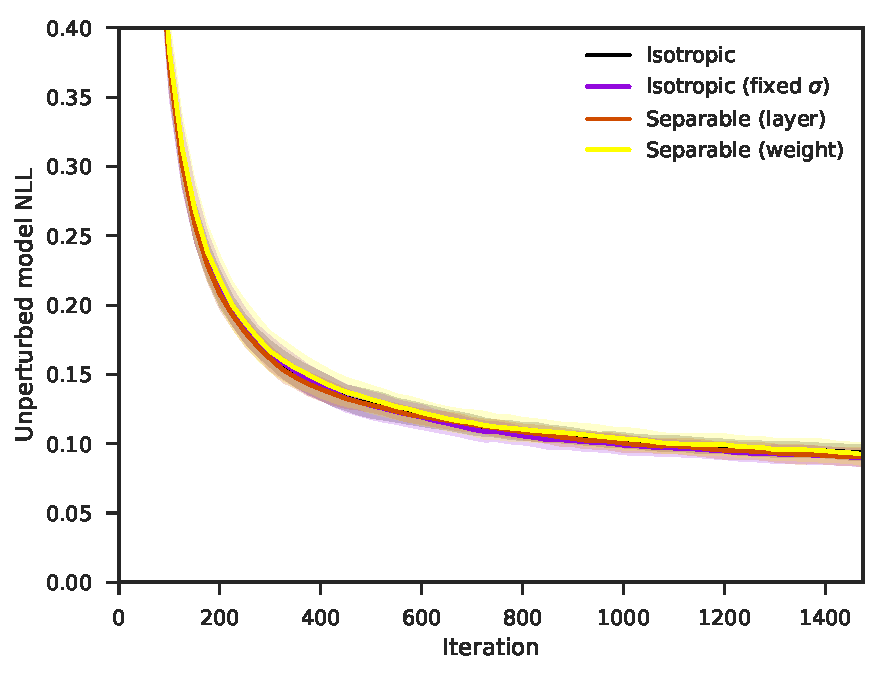
\includegraphics[height=5.8cm]{graphics/E029-VO-S3-analysis-1500/return_val-all-series-mean-sd.pdf}
%         \caption{}
%         \label{fig: Theory: E029-VO-S3-analysis-1500/return_val-all-series-mean-sd}
%     \end{subfigure}
%     \begin{subfigure}[b]{0.49\textwidth}
%         \centering
%         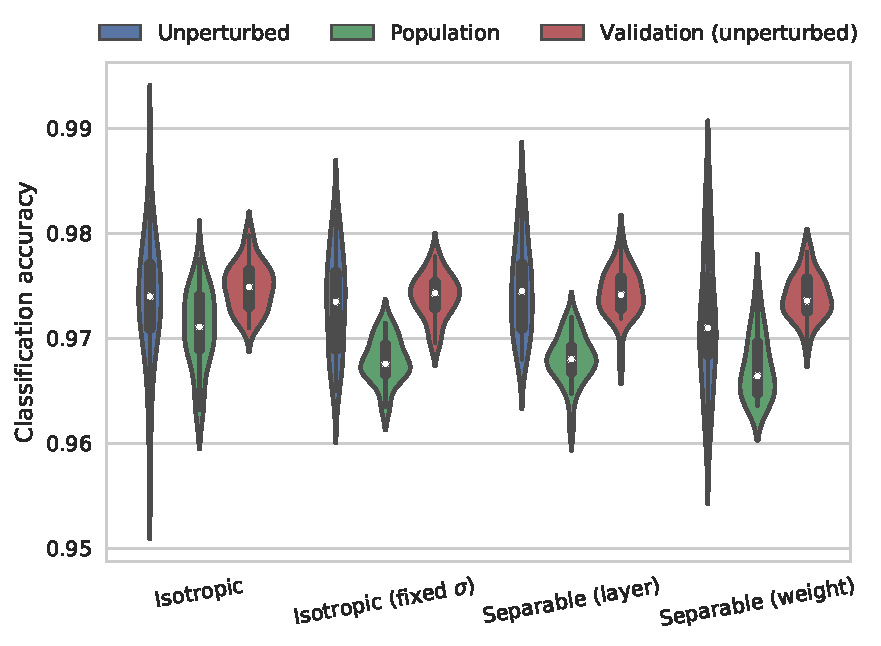
\includegraphics[height=5.3cm]{graphics/E029-VO-S3-analysis-1500/accuracy-final-distribution-boxplot-grouped.pdf}
%         \caption{}
%         \label{fig: Theory: E029-VO-S3-analysis-1500/accuracy-final-distribution-boxplot-grouped}
%     \end{subfigure}
%     \hfill
%     \begin{subfigure}[b]{0.49\textwidth}
%         \centering
%         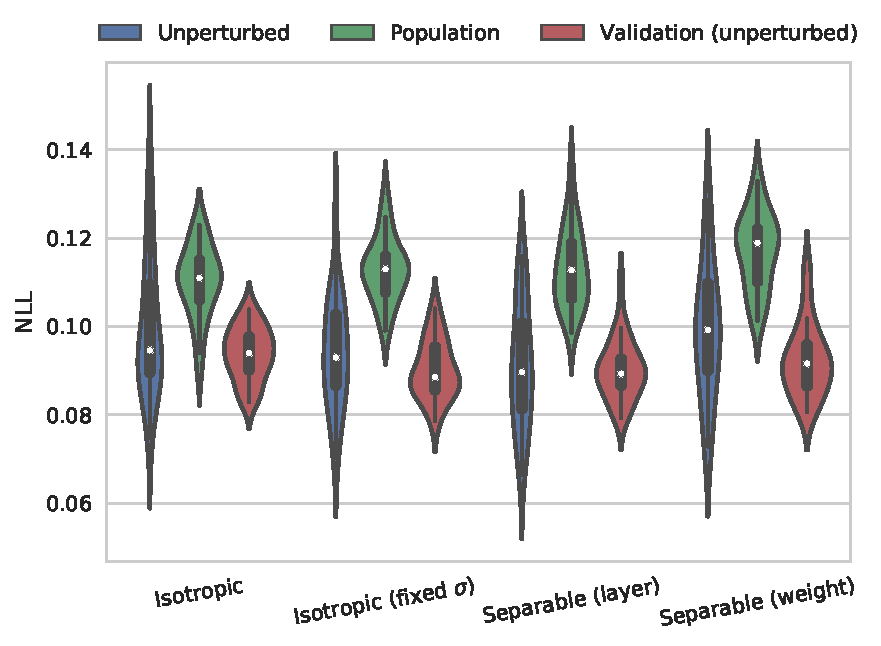
\includegraphics[height=5.3cm]{graphics/E029-VO-S3-analysis-1500/return-final-distribution-boxplot-grouped.pdf}
%         \caption{}
%         \label{fig: Theory: E029-VO-S3-analysis-1500/return-final-distribution-boxplot-grouped}
%     \end{subfigure}
%     \caption{
%         Results of experiments with different \gls{VO} algorithms. The model variations are the fixed variance strategy of \cite{Salimans2017} and \gls{VO} with adjusted variance using an isotropic Gaussian and respectively a layer-wise and per-weight separable Gaussian. Contrary to \cite{Salimans2017}, safe mutation is applied.
%         Plotted versus the iteration number \subref{fig: Theory: E029-VO-S3-analysis-1500/accuracy_val-all-series-mean-sd} shows the validation set classification accuracy and \subref{fig: Theory: E029-VO-S3-analysis-1500/return_val-all-series-mean-sd} the validation set \gls{NLL} loss. 
%         Difference in performance between the algorithms is very small and certainly insignificant.
%         In \subref{fig: Theory: E029-VO-S3-analysis-1500/accuracy-final-distribution-boxplot-grouped} and \subref{fig: Theory: E029-VO-S3-analysis-1500/return-final-distribution-boxplot-grouped} the final distribution of the classification accuracy and \gls{NLL} loss from \subref{fig: Theory: E029-VO-S3-analysis-1500/accuracy_val-all-series-mean-sd} and \subref{fig: Theory: E029-VO-S3-analysis-1500/return_val-all-series-mean-sd} are shown.
%         %These seem to hint at a potential better final performance by adapting the variance of a layer-wise separable Gaussian search distribution.
%         %which is more flexible than an isotropic Gaussian but has fewer parameters and is easier to estimate than a separable Gaussian with per-weight variances.
%     }
%     \label{fig: Theory: E029-VO-S3-analysis-1500}
% \end{figure}


% \begin{figure}[tbp!]
%     \begin{subfigure}[b]{0.49\textwidth}
%         \centering
%         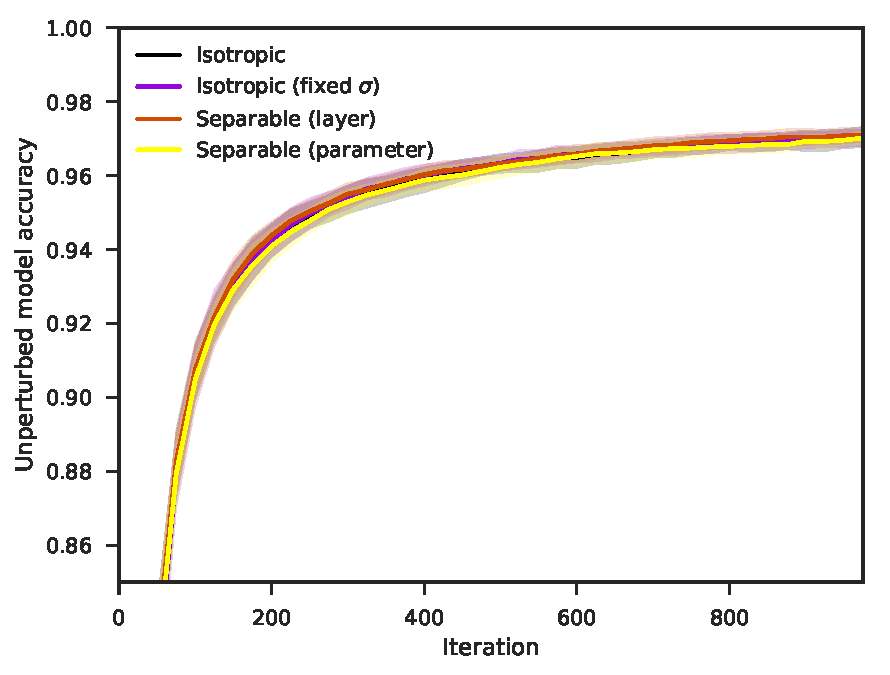
\includegraphics[height=5.8cm]{graphics/E029-VO-S2-analysis/accuracy_val-all-series-mean-sd.pdf}
%         \caption{}
%         \label{fig: Theory: E029-VO-S2-analysis/accuracy_val-all-series-mean-sd}
%     \end{subfigure}
%     \hfill
%     \begin{subfigure}[b]{0.49\textwidth}
%         \centering
%         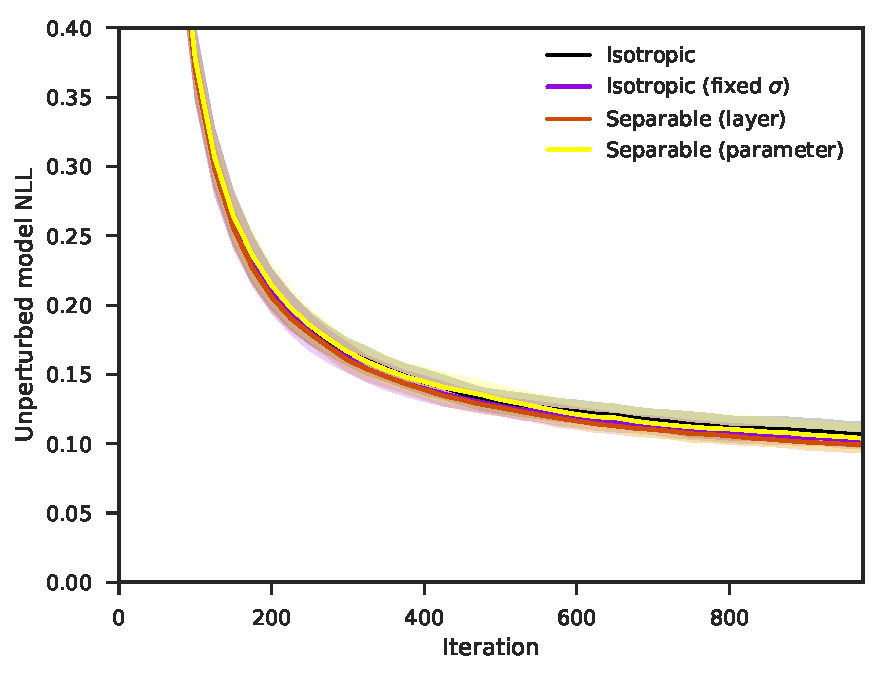
\includegraphics[height=5.8cm]{graphics/E029-VO-S2-analysis/return_val-all-series-mean-sd.pdf}
%         \caption{}
%         \label{fig: Theory: E029-VO-S2-analysis/return_val-all-series-mean-sd}
%     \end{subfigure}
%     \begin{subfigure}[b]{0.49\textwidth}
%         \centering
%         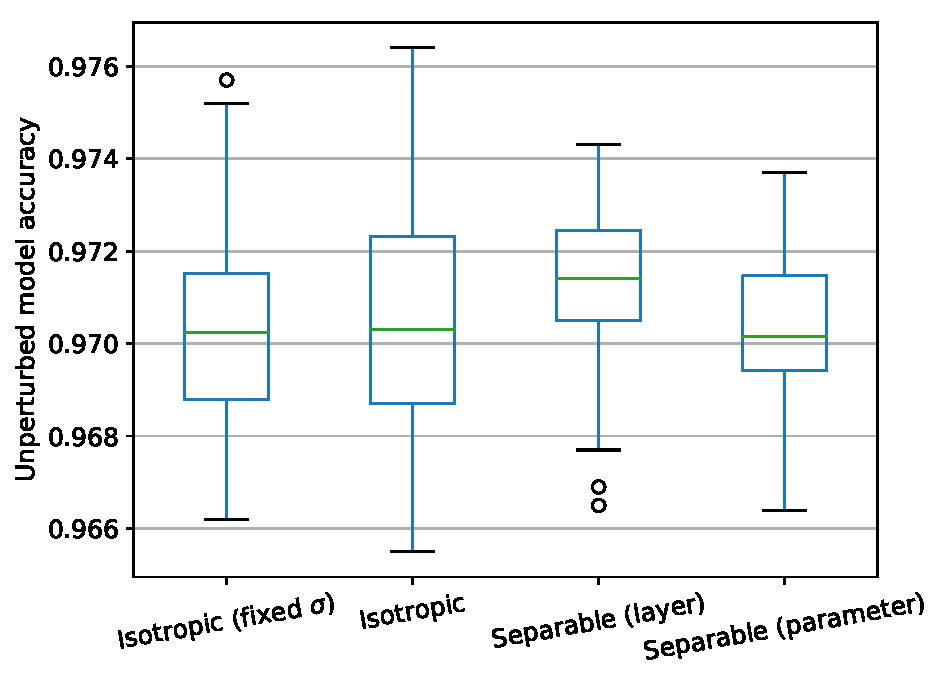
\includegraphics[height=5.2cm]{graphics/E029-VO-S2-analysis/accuracy_val-final-distribution-boxplot.pdf}
%         \caption{}
%         \label{fig: Theory: E029-VO-S2-analysis/accuracy_val-final-distribution-boxplot}
%     \end{subfigure}
%     \hfill
%     \begin{subfigure}[b]{0.49\textwidth}
%         \centering
%         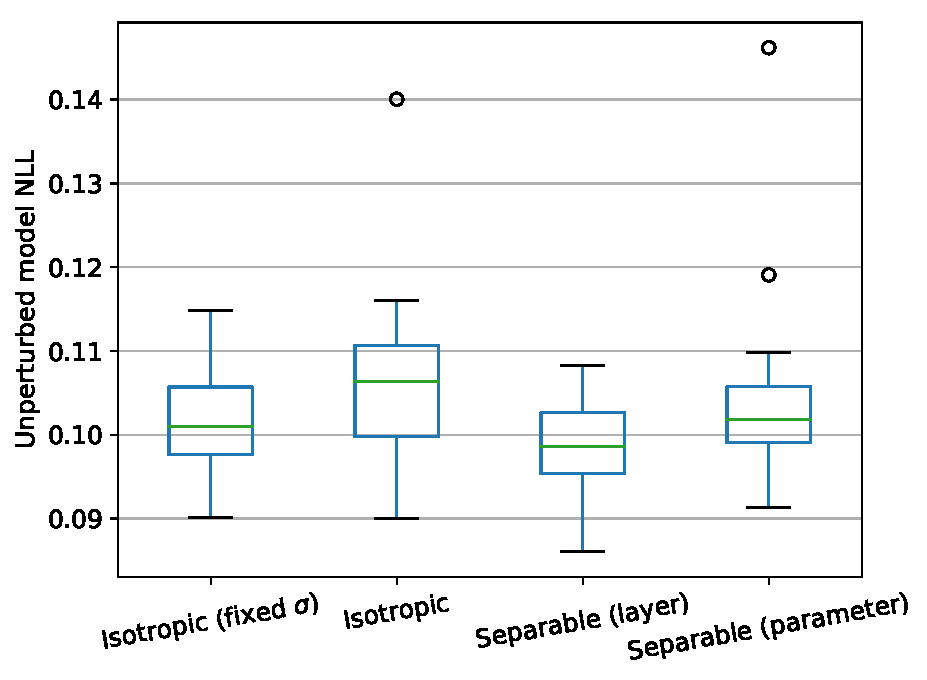
\includegraphics[height=5.2cm]{graphics/E029-VO-S2-analysis/return_val-final-distribution-boxplot.pdf}
%         \caption{}
%         \label{fig: Theory: E029-VO-S2-analysis/return_val-final-distribution-boxplot}
%     \end{subfigure}
%     \caption{
%         Results of experiments with different \gls{VO} algorithms. The plots all show the validation \gls{NLL} or the validation classification accuracy of the unperturbed model. The model variations are the fixed variance strategy of \cite{Salimans2017} and \gls{VO} with adjusted variance using an isotropic Gaussian and respectively a layer-wise and per-weight separable Gaussian.
%         Plotted versus the iteration number \subref{fig: Theory: E029-VO-S2-analysis/accuracy_val-all-series-mean-sd} shows the validation set classification accuracy and \subref{fig: Theory: E029-VO-S2-analysis/return_val-all-series-mean-sd} the validation set \gls{NLL} loss. Difference in performance between the algorithms is very small and certainly insignificant.
%         In \subref{fig: Theory: E029-VO-S2-analysis/accuracy_val-final-distribution-boxplot} and \subref{fig: Theory: E029-VO-S2-analysis/return_val-final-distribution-boxplot} the final distribution of the classification accuracy and \gls{NLL} loss from \subref{fig: Theory: E029-VO-S2-analysis/accuracy_val-all-series-mean-sd} and \subref{fig: Theory: E029-VO-S2-analysis/return_val-all-series-mean-sd} are shown. These seem to hint at a potential better final performance by adapting the variance of a layer-wise separable Gaussian search distribution.
%         %which is more flexible than an isotropic Gaussian but has fewer parameters and is easier to estimate than a separable Gaussian with per-weight variances.
%     }
%     \label{fig: Theory: E029-VO-S2-analysis}
% \end{figure}







\subsection{The gradient norm}
This section examines the interaction between adapting the variance and the norm of the \gls{VO} gradient and the parameter vector in order to shed more light on the effect of adapting the variance. It does so based on single runs of the training, but it should be noted that the observations hold generally for additional runs with different random seeds.

Consider the gradient and parameter norms when using an isotropic Gaussian search distribution. 
As can be seen from the derived \gls{VO} gradient estimators in \eqref{eq: Theory: Variational optimization multivariate isotropic gaussian gradient estimators}, the gradient is scaled by the variance.
In case the variance is fixed, this is obviously a constant scaling factor.
However, when adapting the variance, this effectively scales the term computed by the sum differently at each iteration. It is evident that the variance then has a direct adaptive effect on the gradient norm and thus affects the iteration step size. The effect that the variance has through multiplication on the perturbation and indirectly through the value of the objective function is harder to determine. Since the perturbations are from a standard Gaussian, multiplying them by $\sigma$ does not change their expectation. Additionally, it is theoretically possible for the objective function to both increase and decrease in value for any size of the perturbation. However, very large perturbations must be expected to result in catastrophic forgetting in the perturbed networks as any learned filters etc. are washed out with noise.

\begin{figure}[tbp!]
    \begin{subfigure}[b]{0.49\textwidth}
        \centering
        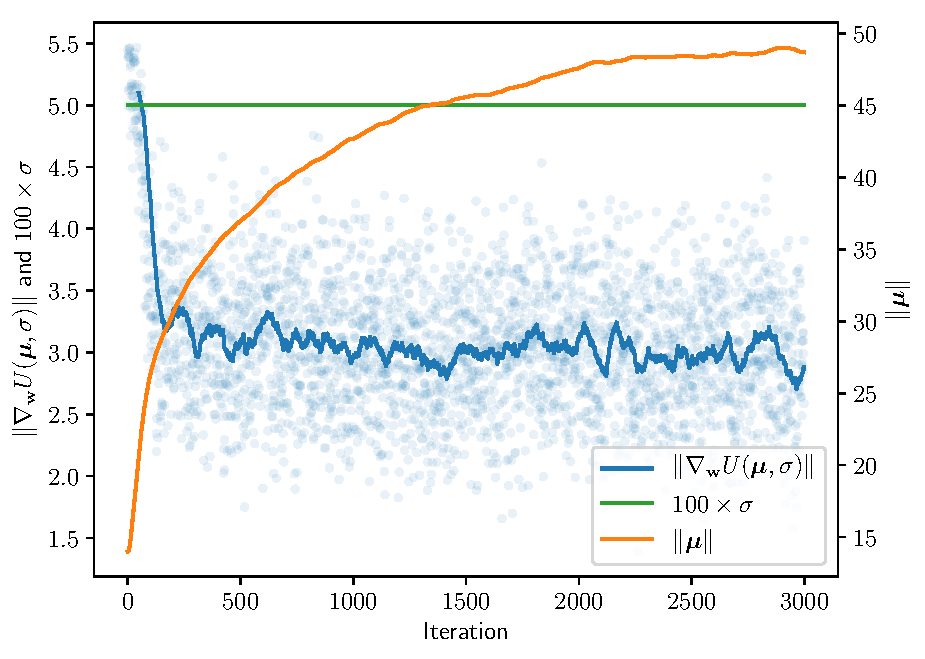
\includegraphics[height=5.5cm]{graphics/E031-NORM-analysis/isotropic-fixed-1-param-and-grad-and-variance-norm.pdf}
        \caption{}
        \label{fig: Theory: E031-NORM-analysis/isotropic-fixed-1-param-and-grad-and-variance-norm}
    \end{subfigure}
    \hfill
    \begin{subfigure}[b]{0.49\textwidth}
        \centering
        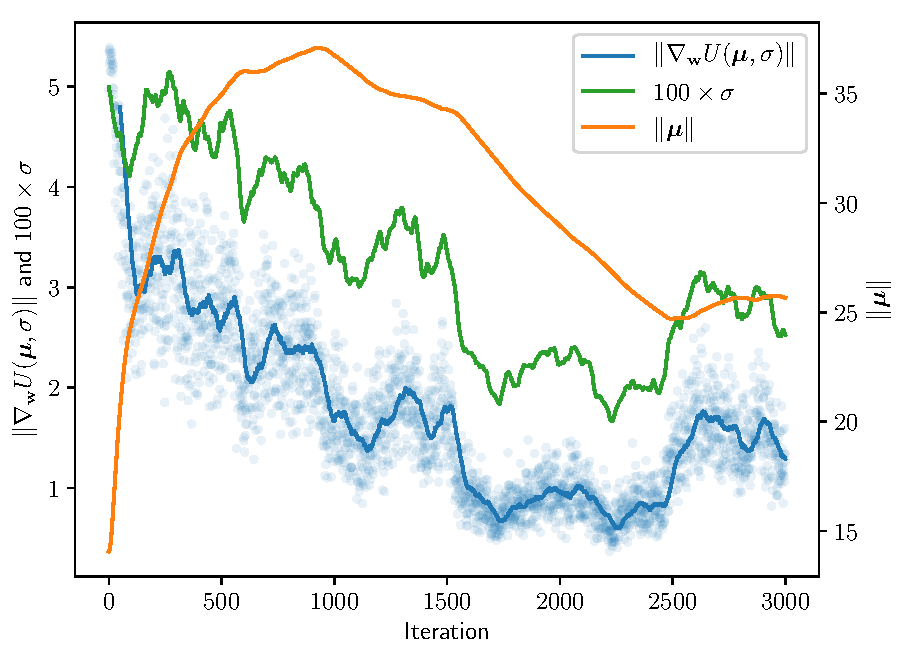
\includegraphics[height=5.5cm]{graphics/E031-NORM-analysis/isotropic-adapted-1-param-and-grad-and-variance-norm.pdf}
        \caption{}
        \label{fig: Theory: E031-NORM-analysis/isotropic-adapted-1-param-and-grad-and-variance-norm}
    \end{subfigure}
    \caption{
        2-norms of the \gls{NN} parameter vector and \gls{VO} gradient for an isotropic Gaussian search distribution with the variance overlayed (multiplied by 100 for scale). In \subref{fig: Theory: E031-NORM-analysis/isotropic-fixed-1-param-and-grad-and-variance-norm} and \subref{fig: Theory: E031-NORM-analysis/isotropic-adapted-1-param-and-grad-and-variance-norm}, the fixed and adapted variance versions are shown, respectively. A centered $50$ sample moving average is computed for the gradient. It is clear that adapting the variance directly and significantly influences the norm of the gradient and in turn also the norm of the parameter vector.
    }
    \label{fig: Theory: E031-NORM-analysis-isotropic}
\end{figure}
The gradient and parameter norms for fixed and adapted variance isotropic Gaussians are plotted in \autoref{fig: Theory: E031-NORM-analysis-isotropic} for a single run of the \gls{MNIST} network (\autoref{lst: Network models: MNIST with batch normalization}). The variance is overlaid in the plots as well. 
A fixed variance (\ref{fig: Theory: E031-NORM-analysis/isotropic-fixed-1-param-and-grad-and-variance-norm}) results in a gradient that rapidly reaches a constant level. The parameter norm increases fairly steadily as a result, but seems to plateau when a minimum is found\footnote{The learning curves are similar to the ones in \autoref{fig: Theory: E029-VO-S5-MD-analysis}}. Interestingly enough, the gradient does not go to zero as the minimum is reached but remains relatively high. This is in-line with the rarity of local minima and the prevalence of saddle points as previously mentioned.
It should be noted that the small amount of $L^2$ regularization adds to decrease the parameter norm. By adapting the variance (\ref{fig: Theory: E031-NORM-analysis/isotropic-adapted-1-param-and-grad-and-variance-norm}), the gradient is also adapted: As the variance decreases so does the gradient norm and in turn the parameter norm as well. The effect of the variance on the gradient norm is similar to that of adaptively decreasing the learning rate during training in the way that increasingly smaller steps are taken as training progresses. By inspecting the results presented in \autoref{fig: Theory: E029-VO-S5-MD-analysis}, it was found that the small poorly performing group of runs that used the adapted isotropic Gaussian had a variance that generally increased rather than decreased throughout training. This then directly resulted in larger gradients and in turn divergence.

\begin{figure}[tbp!]
    \begin{subfigure}[b]{0.49\textwidth}
        \centering
        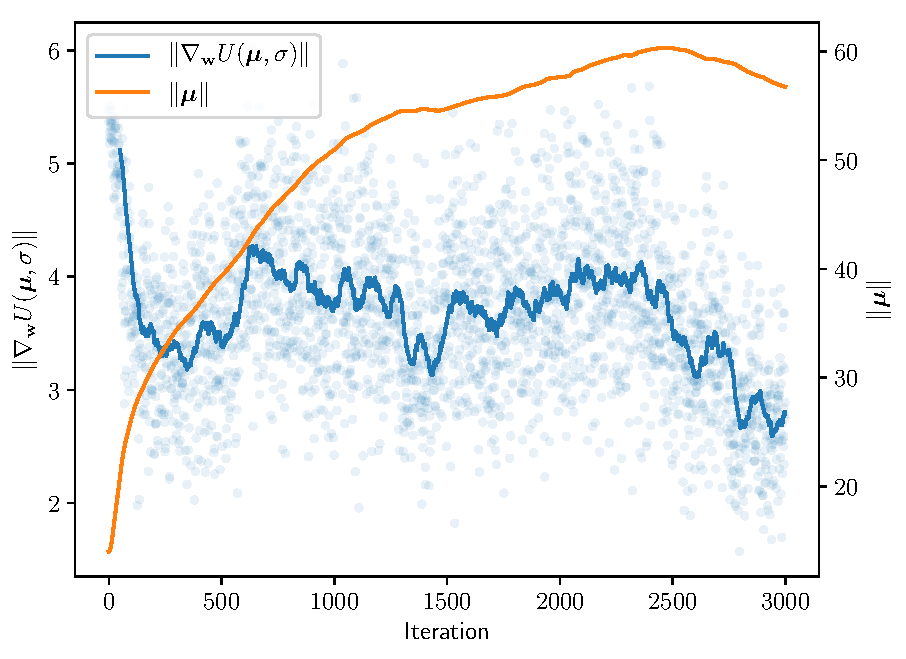
\includegraphics[height=5.6cm]{graphics/E031-NORM-analysis/separable-layer-5-param-and-grad-norm.pdf}
        \caption{}
        \label{fig: Theory: E031-NORM-analysis/separable-layer-5-param-and-grad-norm}
    \end{subfigure}
    \hfill
    \begin{subfigure}[b]{0.49\textwidth}
        \centering
        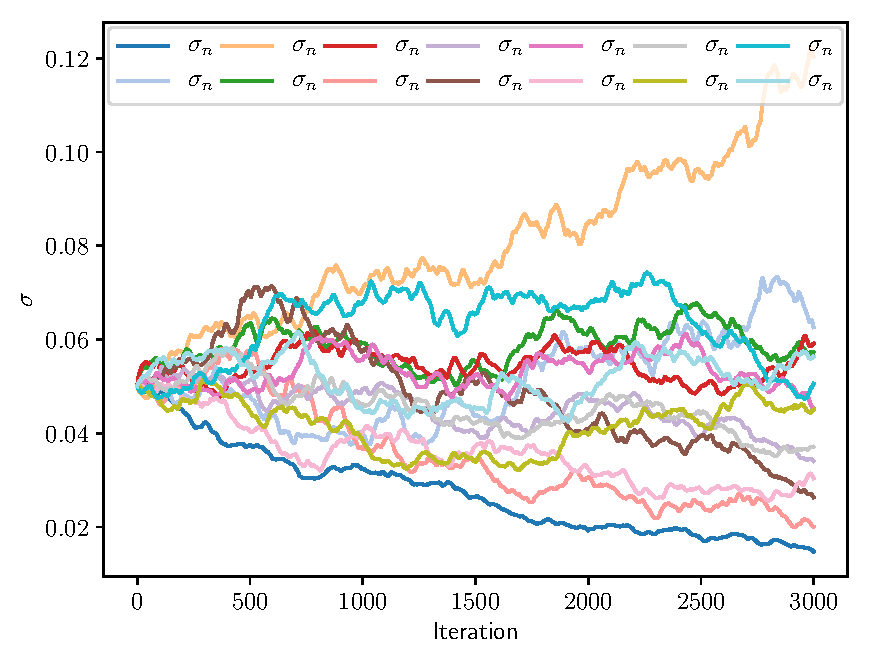
\includegraphics[height=5.6cm]{graphics/E031-NORM-analysis/separable-layer-5-variance.pdf}
        \caption{}
        \label{fig: Theory: E031-NORM-analysis/separable-layer-5-variance}
    \end{subfigure}
    \caption{
        \subref{fig: Theory: E031-NORM-analysis/separable-layer-5-param-and-grad-norm} 2-norms of the \gls{NN} parameter vector and \gls{VO} gradient for a layer-wise separable Gaussian search distribution with the variances plotted separately in \subref{fig: Theory: E031-NORM-analysis/separable-layer-5-variance}. Most variances tend to zero while a few increase. The gradient norm feels the combined effect but generally increases.
    }
    \label{fig: Theory: E031-NORM-analysis-layer-separable}
\end{figure}
\begin{table}[!tbp]
    \centering
    \begin{tabular}{llcc}
\toprule
\# & Layer  & weight/kernel & bias\\
\midrule
1 & Convolutional         &  0  &  1\\
2 & Batch normalization   &  2  &  3\\
3 & Convolutional         &  4  &  5\\
4 & Batch normalization   &  6  &  7\\
5 & Fully connected       &  8  &  9\\
6 & Batch normalization   &  10  &  11\\
7 & Fully connected       &  12  &  13\\
\bottomrule
    \end{tabular}
    \caption{Labels of the variances of the layer-wise separable Gaussian in \autoref{fig: Theory: E031-NORM-analysis-layer-separable} used on the \gls{MNIST} model in \autoref{lst: Network models: MNIST with batch normalization}. The labels are divided into those for the weight/kernel and those for the bias.}
    \label{tab: Experimental work: Adapting the variance}
\end{table}

For the layer-wise separable Gaussians, \autoref{fig: Theory: E031-NORM-analysis-layer-separable} shows the results.
Here, the variances are plotted separately for clarity. 
The variances are labelled incrementally by their layer in the model as described by \autoref{tab: Experimental work: Adapting the variance}. This search distribution often sees many of the variances go toward zero while a few increase.
As for the isotropic case the gradient norm is influenced, but now depends on all the variances. As such it is slightly more smooth but also does not trend as clearly to zero.
One can note that there is some tendency for the variances of earlier layers to decrease more than for later layers. Specifically, the three variances that increase the most are for the \nth{7}, \nth{6} and \nth{5} layer. This can be speculated to be due to the features of earlier layers being learned sooner during training than features of later layers. This might then result in flatter regions of the loss surface in the respective dimensions and thus decreasing variances.

\begin{figure}[tbp!]
    \begin{subfigure}[b]{0.49\textwidth}
        \centering
        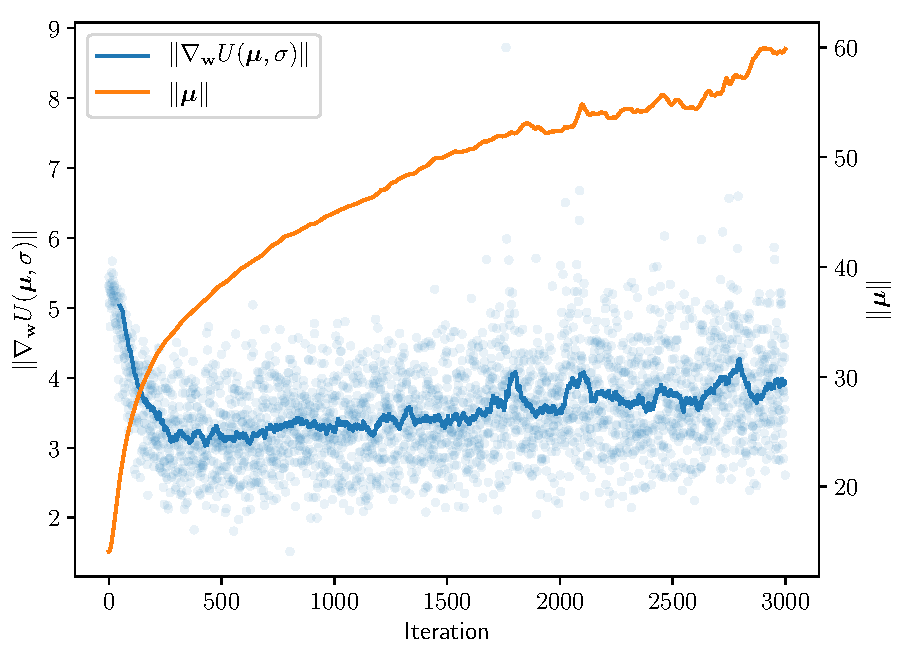
\includegraphics[height=5.6cm]{graphics/E031-NORM-analysis/separable-parameter-1-param-and-grad-norm.pdf}
        \caption{}
        \label{fig: Theory: E031-NORM-analysis/separable-parameter-1-param-and-grad-norm}
    \end{subfigure}
    \hfill
    \begin{subfigure}[b]{0.49\textwidth}
        \centering
        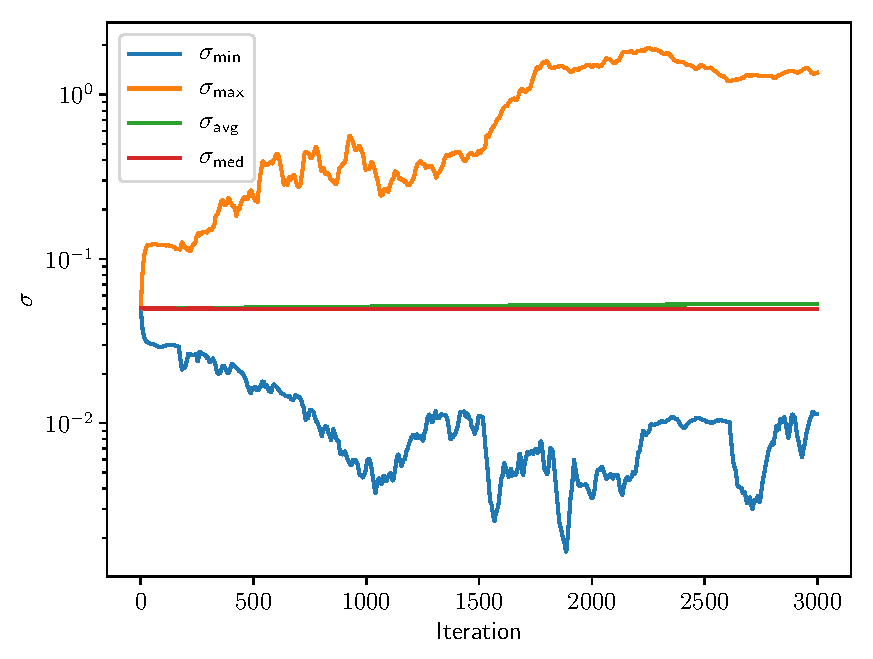
\includegraphics[height=5.6cm]{graphics/E031-NORM-analysis/separable-parameter-1-variance.pdf}
        \caption{}
        \label{fig: Theory: E031-NORM-analysis/separable-parameter-1-variance}
    \end{subfigure}
    \caption{
        \subref{fig: Theory: E031-NORM-analysis/separable-parameter-1-param-and-grad-norm} 2-norms of the \gls{NN} parameter vector and \gls{VO} gradient for a parameter-wise separable Gaussian search distribution with the maximal, minimal, average and median variances plotted separately in \subref{fig: Theory: E031-NORM-analysis/separable-parameter-1-variance}.
    }
    \label{fig: Theory: E031-NORM-analysis-parameter-separable}
\end{figure}
The variances of the parameter-wise separable Gaussian behave similar to the variances of the layer-wise but in a more extreme way and are shown in \autoref{fig: Theory: E031-NORM-analysis-parameter-separable}. The maximal and minimal variances change by two orders of magnitude while the median and average variances remain close to the initial value of $0.5$. The effect on the gradient norm is smaller but there is a tendency for it to increase compared to the fixed variance isotropic Gaussian in \autoref{fig: Theory: E031-NORM-analysis/isotropic-fixed-1-param-and-grad-and-variance-norm}. 
That the parameter-wise variances tend to both increase and decrease by potentially large amounts while the average and median remain approximately at the initial value may indicate that the behaviour is similar to a random walk. 
This behaviour may be due to the fact that many more variance gradients need to be estimated at each iteration while using the same number of perturbations. Additionally, the gradient of the variance of an isotropic Gaussian is estimated by computing the sum of squares of all elements of each perturbation vector. This holds as well for each variance of a layer-wise separable Gaussian considering only the elements used for each layer. In the parameter-wise case however, a single contribution is made from each element of a perturbation vector.
As such, the reason for the random walk behaviour of the variances may be attributable to a poor estimate of their gradients due to a number of effective samples that is too low.


\subsection{Discussion}
The trends in the values of the adapted variances of the separable Gaussians seem to indicate that different layers/parameters have different optimal variances for their perturbations at different times during training. This might help explain why adapting the variance for an isotropic Gaussian sometimes results in divergence while this does not happen for separable Gaussians. When using an isotropic Gaussian, the variance may not be able to appropriately adapt to a wide range of optimal perturbation sizes. Some parameters requiring low variances may then be perturbed with relatively high variance noise and risk losing learned patterns. It should be noted that this is speculative since no experiments have been performed to validate these hypotheses.

The difficulty of drawing benefit from adapting the variance of the search distribution may be partially attributable to the complex geometry of the high dimensional loss surfaces of \glspl{NN}. As previously mentioned, saddle points are exponentially more prevalent than local minima in \gls{NN} loss surfaces while a monotonically decreasing minimization path exists on the loss surface.
The \gls{VO} adapted variance attempts to zero in on a local minimum. It does so by decreasing the variance in regions of high convex curvature and increasing it in regions of low concave curvature.
While the variance is expected to go to zero at a minimum, this is not necessarily the case at a saddle point since only some dimensions exhibit convex curvature.
This is especially obvious in the case of an isotropic Gaussian since this distribution is inherently unable to parameterize differences in the variance between dimensions.
The separable Gaussians allow more such flexibility. This may be a dynamic that adds to the results observed.
Additionally, the monotonically decreasing nature of some paths along the loss surface may encourage a somewhat constant level of the variance, at least in the isotropic case.


\iffalse
Adapting sigma separable per layer seems more stable than both isotropic and per weight. May strike good compromise between flexibility and not too many parameters

How does adapting sigma relate to the shape of the loss surface?

Very steep --> decrease

Very flat --> increase

What if we never reach an area of low gradients?

How about decoupling variance size and learning rate?

\begin{enumerate}
    % \item We may already have established that natural gradient is better so maybe no need for that experiment
    % \item Vanilla ES (VO with single fixed sigma (isotropic)) with importance mixing [include batch normalization, antithetic sampling, fitness shaping and policy network weight decay for comparability]
    % \item VO with single sigma optimization (isotropic) (VO-ISO)
    % \item VO with per layer sigma optimization (separable) (VO-SEP)
    % \item VO with per weight sigma optimization (separable) (VO-SEP)
    \item VO with per layer sigma optimization (full) (VO-COV)
    \item VO with per weight sigma optimization (low rank approx for different $k$) (VO-COV)
    % \item Effect of momentum on sigma gradient (effect of optimizer examined earlier)
    % \item Baseline: back-propagated stochastic gradient descent comparison for \gls{MNIST}
\end{enumerate}

\fi








% \begin{figure}[tbp!]
%     \begin{subfigure}[b]{0.49\textwidth}
%         \centering
%         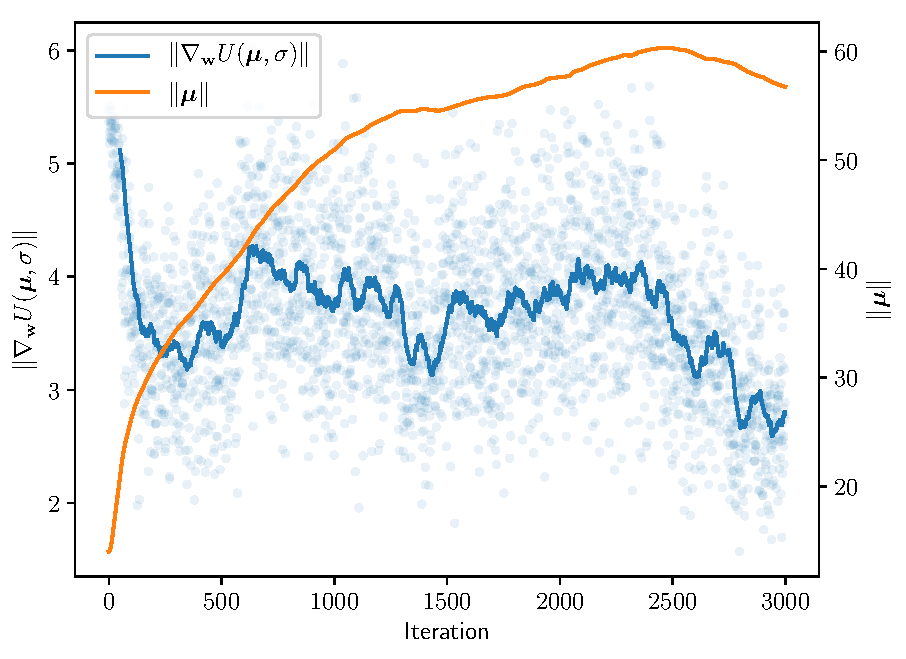
\includegraphics[height=5.6cm]{graphics/E031-NORM-analysis/separable-layer-5-param-and-grad-norm.pdf}
%         \caption{}
%         \label{fig: Theory: E031-NORM-analysis/separable-layer-5-param-and-grad-norm}
%     \end{subfigure}
%     \hfill
%     \begin{subfigure}[b]{0.49\textwidth}
%         \centering
%         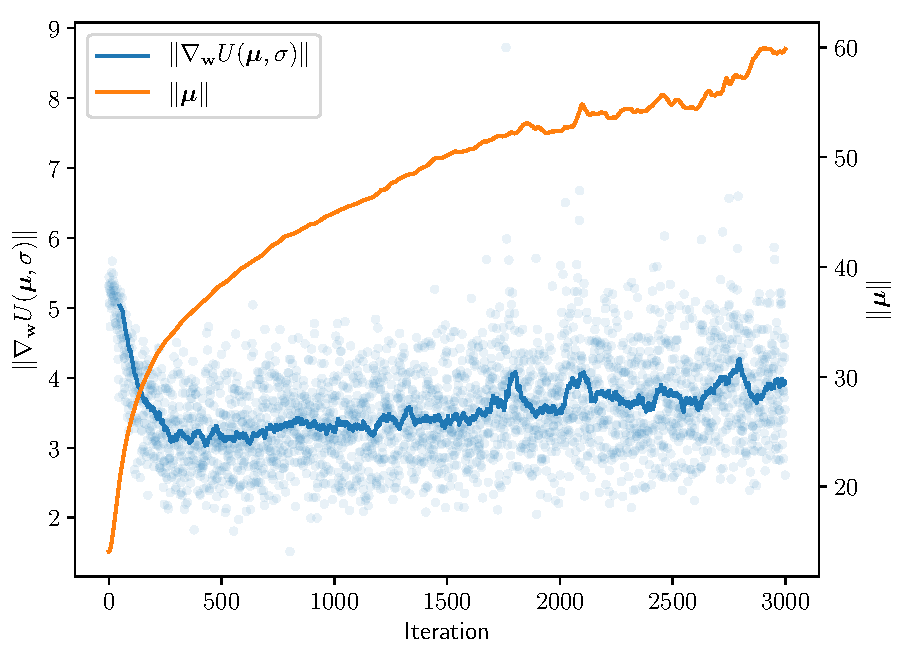
\includegraphics[height=5.6cm]{graphics/E031-NORM-analysis/separable-parameter-1-param-and-grad-norm.pdf}
%         \caption{}
%         \label{fig: Theory: E031-NORM-analysis/separable-parameter-1-param-and-grad-norm}
%     \end{subfigure}
%     \begin{subfigure}[b]{0.49\textwidth}
%         \centering
%         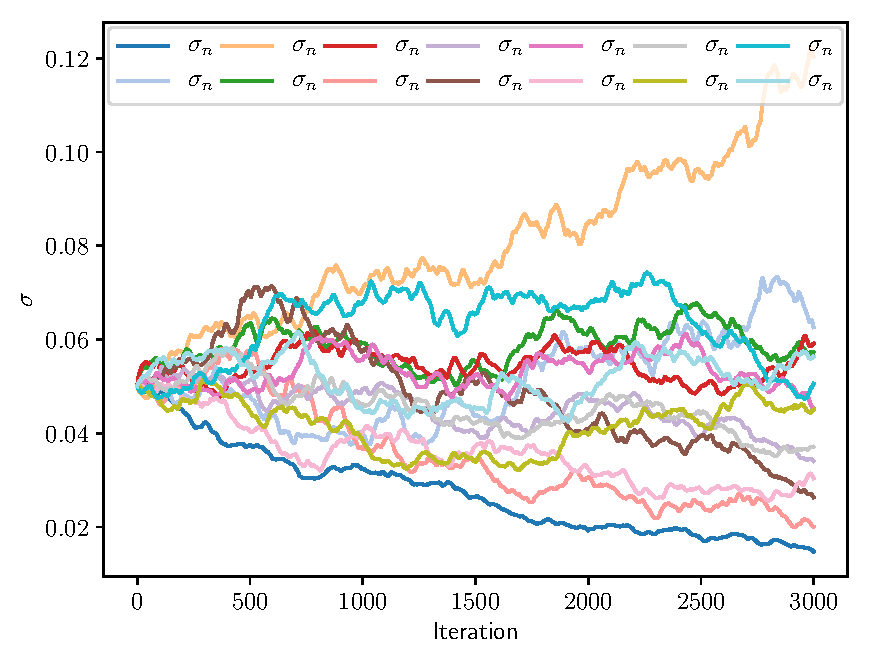
\includegraphics[height=5.8cm]{graphics/E031-NORM-analysis/separable-layer-5-variance.pdf}
%         \caption{}
%         \label{fig: Theory: E031-NORM-analysis/separable-layer-5-variance}
%     \end{subfigure}
%     \hfill
%     \begin{subfigure}[b]{0.49\textwidth}
%         \centering
%         \includegraphics[height=5.8cm]{graphics/E031-NORM-analysis/separable-parameter-1-variance.pdf}
%         \caption{}
%         \label{fig: Theory: E031-NORM-analysis/separable-parameter-1-variance}
%     \end{subfigure}
%     \caption{
%         Results of experiments using \gls{SGD} with momentum on the \gls{VO} gradient for the unperturbed model run on \gls{MNIST}.
%         \subref{fig: Theory: E031-NORM-analysis/isotropic-fixed-1-param-and-grad-and-variance-norm}
%         \subref{fig: Theory: E031-NORM-analysis/isotropic-adapted-1-param-and-grad-and-variance-norm} 
%     }
%     \label{fig: Theory: E031-NORM-analysis}
% \end{figure}

% \begin{figure}[tbp!]
%     \begin{subfigure}[b]{0.49\textwidth}
%         \centering
%         \includegraphics[height=5.8cm]{graphics/E030-MOM-S-analysis/accuracy_unp-all-series-mean-sd.pdf}
%         \caption{}
%         \label{fig: Theory: E030-MOM-S-analysis/accuracy_unp-all-series-mean-sd}
%     \end{subfigure}
%     \hfill
%     \begin{subfigure}[b]{0.49\textwidth}
%         \centering
%         \includegraphics[height=5.8cm]{graphics/E030-MOM-S-analysis/return_unp-all-series-mean-sd.pdf}
%         \caption{}
%         \label{fig: Theory: E030-MOM-S-analysis/return_unp-all-series-mean-sd}
%     \end{subfigure}
%     \caption{
%         Results of experiments using \gls{SGD} with momentum on the \gls{VO} gradient for the unperturbed model run on \gls{MNIST}.
%         \subref{fig: Theory: E030-MOM-S-analysis/accuracy_unp-all-series-mean-sd} Training and validation set classification accuracy.
%         \subref{fig: Theory: E030-MOM-S-analysis/return_unp-all-series-mean-sd} Training and validation set \gls{NLL} loss.
%     }
%     \label{fig: Theory: E030-MOM-S-analysis}
% \end{figure}







